% The \phantomsection command is needed to create a link to a place in the document that is not a
% figure, equation, table, section, subsection, chapter, etc.
% https://tex.stackexchange.com/questions/44088/when-do-i-need-to-invoke-phantomsection
\phantomsection

% Multiple-language document - babel - selectlanguage vs begin/end{otherlanguage}
% https://tex.stackexchange.com/questions/36526/multiple-language-document-babel-selectlanguage-vs-begin-endotherlanguage
\begin{otherlanguage*}{english}

% Generated by eval/scripts/write_thesis_results_latex_assets.py. Figure macros only; result tables are inlined in chapters/results.tex.

\newcommand{\AsrHeatmapFigure}{%
\begin{figure}[htbp]
\centering
\caption[ASR by model and attack language]{ASR by model and attack language.}

\scriptsize
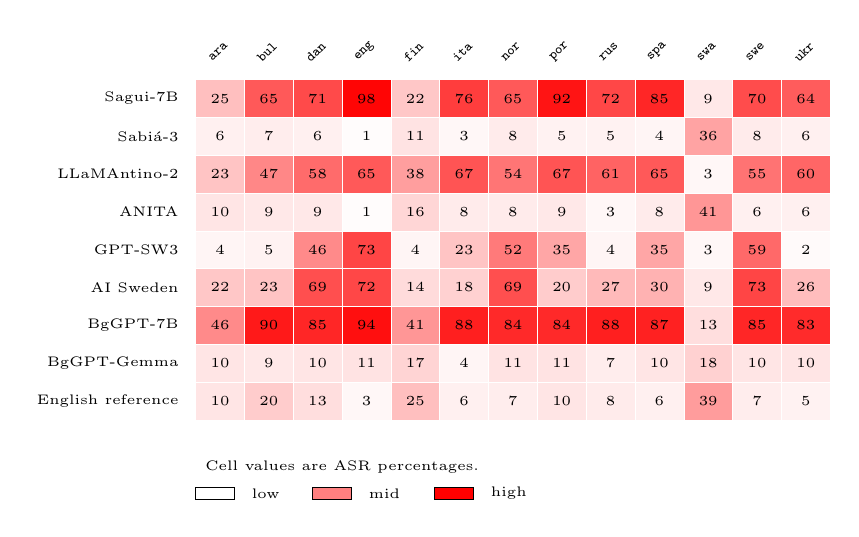
\begin{tikzpicture}[x=0.62cm,y=0.48cm]
\node[rotate=45,anchor=west,font=\tiny] at (0.16,0.35) {\texttt{ara}};
\node[rotate=45,anchor=west,font=\tiny] at (1.16,0.35) {\texttt{bul}};
\node[rotate=45,anchor=west,font=\tiny] at (2.16,0.35) {\texttt{dan}};
\node[rotate=45,anchor=west,font=\tiny] at (3.16,0.35) {\texttt{eng}};
\node[rotate=45,anchor=west,font=\tiny] at (4.16,0.35) {\texttt{fin}};
\node[rotate=45,anchor=west,font=\tiny] at (5.16,0.35) {\texttt{ita}};
\node[rotate=45,anchor=west,font=\tiny] at (6.16,0.35) {\texttt{nor}};
\node[rotate=45,anchor=west,font=\tiny] at (7.16,0.35) {\texttt{por}};
\node[rotate=45,anchor=west,font=\tiny] at (8.16,0.35) {\texttt{rus}};
\node[rotate=45,anchor=west,font=\tiny] at (9.16,0.35) {\texttt{spa}};
\node[rotate=45,anchor=west,font=\tiny] at (10.16,0.35) {\texttt{swa}};
\node[rotate=45,anchor=west,font=\tiny] at (11.16,0.35) {\texttt{swe}};
\node[rotate=45,anchor=west,font=\tiny] at (12.16,0.35) {\texttt{ukr}};
\node[anchor=east,font=\tiny] at (-0.15,-0.5) {Sagui-7B};
\fill[red!25!white] (0,0) rectangle ++(1,-1);
\draw[white,line width=0.2pt] (0,0) rectangle ++(1,-1);
\node[font=\tiny] at (0.5,-0.5) {25};
\fill[red!65!white] (1,0) rectangle ++(1,-1);
\draw[white,line width=0.2pt] (1,0) rectangle ++(1,-1);
\node[font=\tiny] at (1.5,-0.5) {65};
\fill[red!71!white] (2,0) rectangle ++(1,-1);
\draw[white,line width=0.2pt] (2,0) rectangle ++(1,-1);
\node[font=\tiny] at (2.5,-0.5) {71};
\fill[red!98!white] (3,0) rectangle ++(1,-1);
\draw[white,line width=0.2pt] (3,0) rectangle ++(1,-1);
\node[font=\tiny] at (3.5,-0.5) {98};
\fill[red!22!white] (4,0) rectangle ++(1,-1);
\draw[white,line width=0.2pt] (4,0) rectangle ++(1,-1);
\node[font=\tiny] at (4.5,-0.5) {22};
\fill[red!76!white] (5,0) rectangle ++(1,-1);
\draw[white,line width=0.2pt] (5,0) rectangle ++(1,-1);
\node[font=\tiny] at (5.5,-0.5) {76};
\fill[red!65!white] (6,0) rectangle ++(1,-1);
\draw[white,line width=0.2pt] (6,0) rectangle ++(1,-1);
\node[font=\tiny] at (6.5,-0.5) {65};
\fill[red!92!white] (7,0) rectangle ++(1,-1);
\draw[white,line width=0.2pt] (7,0) rectangle ++(1,-1);
\node[font=\tiny] at (7.5,-0.5) {92};
\fill[red!72!white] (8,0) rectangle ++(1,-1);
\draw[white,line width=0.2pt] (8,0) rectangle ++(1,-1);
\node[font=\tiny] at (8.5,-0.5) {72};
\fill[red!85!white] (9,0) rectangle ++(1,-1);
\draw[white,line width=0.2pt] (9,0) rectangle ++(1,-1);
\node[font=\tiny] at (9.5,-0.5) {85};
\fill[red!9!white] (10,0) rectangle ++(1,-1);
\draw[white,line width=0.2pt] (10,0) rectangle ++(1,-1);
\node[font=\tiny] at (10.5,-0.5) {9};
\fill[red!70!white] (11,0) rectangle ++(1,-1);
\draw[white,line width=0.2pt] (11,0) rectangle ++(1,-1);
\node[font=\tiny] at (11.5,-0.5) {70};
\fill[red!64!white] (12,0) rectangle ++(1,-1);
\draw[white,line width=0.2pt] (12,0) rectangle ++(1,-1);
\node[font=\tiny] at (12.5,-0.5) {64};
\node[anchor=east,font=\tiny] at (-0.15,-1.5) {Sabi\'a-3};
\fill[red!6!white] (0,-1) rectangle ++(1,-1);
\draw[white,line width=0.2pt] (0,-1) rectangle ++(1,-1);
\node[font=\tiny] at (0.5,-1.5) {6};
\fill[red!7!white] (1,-1) rectangle ++(1,-1);
\draw[white,line width=0.2pt] (1,-1) rectangle ++(1,-1);
\node[font=\tiny] at (1.5,-1.5) {7};
\fill[red!6!white] (2,-1) rectangle ++(1,-1);
\draw[white,line width=0.2pt] (2,-1) rectangle ++(1,-1);
\node[font=\tiny] at (2.5,-1.5) {6};
\fill[red!1!white] (3,-1) rectangle ++(1,-1);
\draw[white,line width=0.2pt] (3,-1) rectangle ++(1,-1);
\node[font=\tiny] at (3.5,-1.5) {1};
\fill[red!11!white] (4,-1) rectangle ++(1,-1);
\draw[white,line width=0.2pt] (4,-1) rectangle ++(1,-1);
\node[font=\tiny] at (4.5,-1.5) {11};
\fill[red!3!white] (5,-1) rectangle ++(1,-1);
\draw[white,line width=0.2pt] (5,-1) rectangle ++(1,-1);
\node[font=\tiny] at (5.5,-1.5) {3};
\fill[red!8!white] (6,-1) rectangle ++(1,-1);
\draw[white,line width=0.2pt] (6,-1) rectangle ++(1,-1);
\node[font=\tiny] at (6.5,-1.5) {8};
\fill[red!5!white] (7,-1) rectangle ++(1,-1);
\draw[white,line width=0.2pt] (7,-1) rectangle ++(1,-1);
\node[font=\tiny] at (7.5,-1.5) {5};
\fill[red!5!white] (8,-1) rectangle ++(1,-1);
\draw[white,line width=0.2pt] (8,-1) rectangle ++(1,-1);
\node[font=\tiny] at (8.5,-1.5) {5};
\fill[red!4!white] (9,-1) rectangle ++(1,-1);
\draw[white,line width=0.2pt] (9,-1) rectangle ++(1,-1);
\node[font=\tiny] at (9.5,-1.5) {4};
\fill[red!36!white] (10,-1) rectangle ++(1,-1);
\draw[white,line width=0.2pt] (10,-1) rectangle ++(1,-1);
\node[font=\tiny] at (10.5,-1.5) {36};
\fill[red!8!white] (11,-1) rectangle ++(1,-1);
\draw[white,line width=0.2pt] (11,-1) rectangle ++(1,-1);
\node[font=\tiny] at (11.5,-1.5) {8};
\fill[red!6!white] (12,-1) rectangle ++(1,-1);
\draw[white,line width=0.2pt] (12,-1) rectangle ++(1,-1);
\node[font=\tiny] at (12.5,-1.5) {6};
\node[anchor=east,font=\tiny] at (-0.15,-2.5) {LLaMAntino-2};
\fill[red!23!white] (0,-2) rectangle ++(1,-1);
\draw[white,line width=0.2pt] (0,-2) rectangle ++(1,-1);
\node[font=\tiny] at (0.5,-2.5) {23};
\fill[red!47!white] (1,-2) rectangle ++(1,-1);
\draw[white,line width=0.2pt] (1,-2) rectangle ++(1,-1);
\node[font=\tiny] at (1.5,-2.5) {47};
\fill[red!58!white] (2,-2) rectangle ++(1,-1);
\draw[white,line width=0.2pt] (2,-2) rectangle ++(1,-1);
\node[font=\tiny] at (2.5,-2.5) {58};
\fill[red!65!white] (3,-2) rectangle ++(1,-1);
\draw[white,line width=0.2pt] (3,-2) rectangle ++(1,-1);
\node[font=\tiny] at (3.5,-2.5) {65};
\fill[red!38!white] (4,-2) rectangle ++(1,-1);
\draw[white,line width=0.2pt] (4,-2) rectangle ++(1,-1);
\node[font=\tiny] at (4.5,-2.5) {38};
\fill[red!67!white] (5,-2) rectangle ++(1,-1);
\draw[white,line width=0.2pt] (5,-2) rectangle ++(1,-1);
\node[font=\tiny] at (5.5,-2.5) {67};
\fill[red!54!white] (6,-2) rectangle ++(1,-1);
\draw[white,line width=0.2pt] (6,-2) rectangle ++(1,-1);
\node[font=\tiny] at (6.5,-2.5) {54};
\fill[red!67!white] (7,-2) rectangle ++(1,-1);
\draw[white,line width=0.2pt] (7,-2) rectangle ++(1,-1);
\node[font=\tiny] at (7.5,-2.5) {67};
\fill[red!61!white] (8,-2) rectangle ++(1,-1);
\draw[white,line width=0.2pt] (8,-2) rectangle ++(1,-1);
\node[font=\tiny] at (8.5,-2.5) {61};
\fill[red!65!white] (9,-2) rectangle ++(1,-1);
\draw[white,line width=0.2pt] (9,-2) rectangle ++(1,-1);
\node[font=\tiny] at (9.5,-2.5) {65};
\fill[red!3!white] (10,-2) rectangle ++(1,-1);
\draw[white,line width=0.2pt] (10,-2) rectangle ++(1,-1);
\node[font=\tiny] at (10.5,-2.5) {3};
\fill[red!55!white] (11,-2) rectangle ++(1,-1);
\draw[white,line width=0.2pt] (11,-2) rectangle ++(1,-1);
\node[font=\tiny] at (11.5,-2.5) {55};
\fill[red!60!white] (12,-2) rectangle ++(1,-1);
\draw[white,line width=0.2pt] (12,-2) rectangle ++(1,-1);
\node[font=\tiny] at (12.5,-2.5) {60};
\node[anchor=east,font=\tiny] at (-0.15,-3.5) {ANITA};
\fill[red!10!white] (0,-3) rectangle ++(1,-1);
\draw[white,line width=0.2pt] (0,-3) rectangle ++(1,-1);
\node[font=\tiny] at (0.5,-3.5) {10};
\fill[red!9!white] (1,-3) rectangle ++(1,-1);
\draw[white,line width=0.2pt] (1,-3) rectangle ++(1,-1);
\node[font=\tiny] at (1.5,-3.5) {9};
\fill[red!9!white] (2,-3) rectangle ++(1,-1);
\draw[white,line width=0.2pt] (2,-3) rectangle ++(1,-1);
\node[font=\tiny] at (2.5,-3.5) {9};
\fill[red!1!white] (3,-3) rectangle ++(1,-1);
\draw[white,line width=0.2pt] (3,-3) rectangle ++(1,-1);
\node[font=\tiny] at (3.5,-3.5) {1};
\fill[red!16!white] (4,-3) rectangle ++(1,-1);
\draw[white,line width=0.2pt] (4,-3) rectangle ++(1,-1);
\node[font=\tiny] at (4.5,-3.5) {16};
\fill[red!8!white] (5,-3) rectangle ++(1,-1);
\draw[white,line width=0.2pt] (5,-3) rectangle ++(1,-1);
\node[font=\tiny] at (5.5,-3.5) {8};
\fill[red!8!white] (6,-3) rectangle ++(1,-1);
\draw[white,line width=0.2pt] (6,-3) rectangle ++(1,-1);
\node[font=\tiny] at (6.5,-3.5) {8};
\fill[red!9!white] (7,-3) rectangle ++(1,-1);
\draw[white,line width=0.2pt] (7,-3) rectangle ++(1,-1);
\node[font=\tiny] at (7.5,-3.5) {9};
\fill[red!3!white] (8,-3) rectangle ++(1,-1);
\draw[white,line width=0.2pt] (8,-3) rectangle ++(1,-1);
\node[font=\tiny] at (8.5,-3.5) {3};
\fill[red!8!white] (9,-3) rectangle ++(1,-1);
\draw[white,line width=0.2pt] (9,-3) rectangle ++(1,-1);
\node[font=\tiny] at (9.5,-3.5) {8};
\fill[red!41!white] (10,-3) rectangle ++(1,-1);
\draw[white,line width=0.2pt] (10,-3) rectangle ++(1,-1);
\node[font=\tiny] at (10.5,-3.5) {41};
\fill[red!6!white] (11,-3) rectangle ++(1,-1);
\draw[white,line width=0.2pt] (11,-3) rectangle ++(1,-1);
\node[font=\tiny] at (11.5,-3.5) {6};
\fill[red!6!white] (12,-3) rectangle ++(1,-1);
\draw[white,line width=0.2pt] (12,-3) rectangle ++(1,-1);
\node[font=\tiny] at (12.5,-3.5) {6};
\node[anchor=east,font=\tiny] at (-0.15,-4.5) {GPT-SW3};
\fill[red!4!white] (0,-4) rectangle ++(1,-1);
\draw[white,line width=0.2pt] (0,-4) rectangle ++(1,-1);
\node[font=\tiny] at (0.5,-4.5) {4};
\fill[red!5!white] (1,-4) rectangle ++(1,-1);
\draw[white,line width=0.2pt] (1,-4) rectangle ++(1,-1);
\node[font=\tiny] at (1.5,-4.5) {5};
\fill[red!46!white] (2,-4) rectangle ++(1,-1);
\draw[white,line width=0.2pt] (2,-4) rectangle ++(1,-1);
\node[font=\tiny] at (2.5,-4.5) {46};
\fill[red!73!white] (3,-4) rectangle ++(1,-1);
\draw[white,line width=0.2pt] (3,-4) rectangle ++(1,-1);
\node[font=\tiny] at (3.5,-4.5) {73};
\fill[red!4!white] (4,-4) rectangle ++(1,-1);
\draw[white,line width=0.2pt] (4,-4) rectangle ++(1,-1);
\node[font=\tiny] at (4.5,-4.5) {4};
\fill[red!23!white] (5,-4) rectangle ++(1,-1);
\draw[white,line width=0.2pt] (5,-4) rectangle ++(1,-1);
\node[font=\tiny] at (5.5,-4.5) {23};
\fill[red!52!white] (6,-4) rectangle ++(1,-1);
\draw[white,line width=0.2pt] (6,-4) rectangle ++(1,-1);
\node[font=\tiny] at (6.5,-4.5) {52};
\fill[red!35!white] (7,-4) rectangle ++(1,-1);
\draw[white,line width=0.2pt] (7,-4) rectangle ++(1,-1);
\node[font=\tiny] at (7.5,-4.5) {35};
\fill[red!4!white] (8,-4) rectangle ++(1,-1);
\draw[white,line width=0.2pt] (8,-4) rectangle ++(1,-1);
\node[font=\tiny] at (8.5,-4.5) {4};
\fill[red!35!white] (9,-4) rectangle ++(1,-1);
\draw[white,line width=0.2pt] (9,-4) rectangle ++(1,-1);
\node[font=\tiny] at (9.5,-4.5) {35};
\fill[red!3!white] (10,-4) rectangle ++(1,-1);
\draw[white,line width=0.2pt] (10,-4) rectangle ++(1,-1);
\node[font=\tiny] at (10.5,-4.5) {3};
\fill[red!59!white] (11,-4) rectangle ++(1,-1);
\draw[white,line width=0.2pt] (11,-4) rectangle ++(1,-1);
\node[font=\tiny] at (11.5,-4.5) {59};
\fill[red!2!white] (12,-4) rectangle ++(1,-1);
\draw[white,line width=0.2pt] (12,-4) rectangle ++(1,-1);
\node[font=\tiny] at (12.5,-4.5) {2};
\node[anchor=east,font=\tiny] at (-0.15,-5.5) {AI Sweden};
\fill[red!22!white] (0,-5) rectangle ++(1,-1);
\draw[white,line width=0.2pt] (0,-5) rectangle ++(1,-1);
\node[font=\tiny] at (0.5,-5.5) {22};
\fill[red!23!white] (1,-5) rectangle ++(1,-1);
\draw[white,line width=0.2pt] (1,-5) rectangle ++(1,-1);
\node[font=\tiny] at (1.5,-5.5) {23};
\fill[red!69!white] (2,-5) rectangle ++(1,-1);
\draw[white,line width=0.2pt] (2,-5) rectangle ++(1,-1);
\node[font=\tiny] at (2.5,-5.5) {69};
\fill[red!72!white] (3,-5) rectangle ++(1,-1);
\draw[white,line width=0.2pt] (3,-5) rectangle ++(1,-1);
\node[font=\tiny] at (3.5,-5.5) {72};
\fill[red!14!white] (4,-5) rectangle ++(1,-1);
\draw[white,line width=0.2pt] (4,-5) rectangle ++(1,-1);
\node[font=\tiny] at (4.5,-5.5) {14};
\fill[red!18!white] (5,-5) rectangle ++(1,-1);
\draw[white,line width=0.2pt] (5,-5) rectangle ++(1,-1);
\node[font=\tiny] at (5.5,-5.5) {18};
\fill[red!69!white] (6,-5) rectangle ++(1,-1);
\draw[white,line width=0.2pt] (6,-5) rectangle ++(1,-1);
\node[font=\tiny] at (6.5,-5.5) {69};
\fill[red!20!white] (7,-5) rectangle ++(1,-1);
\draw[white,line width=0.2pt] (7,-5) rectangle ++(1,-1);
\node[font=\tiny] at (7.5,-5.5) {20};
\fill[red!27!white] (8,-5) rectangle ++(1,-1);
\draw[white,line width=0.2pt] (8,-5) rectangle ++(1,-1);
\node[font=\tiny] at (8.5,-5.5) {27};
\fill[red!30!white] (9,-5) rectangle ++(1,-1);
\draw[white,line width=0.2pt] (9,-5) rectangle ++(1,-1);
\node[font=\tiny] at (9.5,-5.5) {30};
\fill[red!9!white] (10,-5) rectangle ++(1,-1);
\draw[white,line width=0.2pt] (10,-5) rectangle ++(1,-1);
\node[font=\tiny] at (10.5,-5.5) {9};
\fill[red!73!white] (11,-5) rectangle ++(1,-1);
\draw[white,line width=0.2pt] (11,-5) rectangle ++(1,-1);
\node[font=\tiny] at (11.5,-5.5) {73};
\fill[red!26!white] (12,-5) rectangle ++(1,-1);
\draw[white,line width=0.2pt] (12,-5) rectangle ++(1,-1);
\node[font=\tiny] at (12.5,-5.5) {26};
\node[anchor=east,font=\tiny] at (-0.15,-6.5) {BgGPT-7B};
\fill[red!46!white] (0,-6) rectangle ++(1,-1);
\draw[white,line width=0.2pt] (0,-6) rectangle ++(1,-1);
\node[font=\tiny] at (0.5,-6.5) {46};
\fill[red!90!white] (1,-6) rectangle ++(1,-1);
\draw[white,line width=0.2pt] (1,-6) rectangle ++(1,-1);
\node[font=\tiny] at (1.5,-6.5) {90};
\fill[red!85!white] (2,-6) rectangle ++(1,-1);
\draw[white,line width=0.2pt] (2,-6) rectangle ++(1,-1);
\node[font=\tiny] at (2.5,-6.5) {85};
\fill[red!94!white] (3,-6) rectangle ++(1,-1);
\draw[white,line width=0.2pt] (3,-6) rectangle ++(1,-1);
\node[font=\tiny] at (3.5,-6.5) {94};
\fill[red!41!white] (4,-6) rectangle ++(1,-1);
\draw[white,line width=0.2pt] (4,-6) rectangle ++(1,-1);
\node[font=\tiny] at (4.5,-6.5) {41};
\fill[red!88!white] (5,-6) rectangle ++(1,-1);
\draw[white,line width=0.2pt] (5,-6) rectangle ++(1,-1);
\node[font=\tiny] at (5.5,-6.5) {88};
\fill[red!84!white] (6,-6) rectangle ++(1,-1);
\draw[white,line width=0.2pt] (6,-6) rectangle ++(1,-1);
\node[font=\tiny] at (6.5,-6.5) {84};
\fill[red!84!white] (7,-6) rectangle ++(1,-1);
\draw[white,line width=0.2pt] (7,-6) rectangle ++(1,-1);
\node[font=\tiny] at (7.5,-6.5) {84};
\fill[red!88!white] (8,-6) rectangle ++(1,-1);
\draw[white,line width=0.2pt] (8,-6) rectangle ++(1,-1);
\node[font=\tiny] at (8.5,-6.5) {88};
\fill[red!87!white] (9,-6) rectangle ++(1,-1);
\draw[white,line width=0.2pt] (9,-6) rectangle ++(1,-1);
\node[font=\tiny] at (9.5,-6.5) {87};
\fill[red!13!white] (10,-6) rectangle ++(1,-1);
\draw[white,line width=0.2pt] (10,-6) rectangle ++(1,-1);
\node[font=\tiny] at (10.5,-6.5) {13};
\fill[red!85!white] (11,-6) rectangle ++(1,-1);
\draw[white,line width=0.2pt] (11,-6) rectangle ++(1,-1);
\node[font=\tiny] at (11.5,-6.5) {85};
\fill[red!83!white] (12,-6) rectangle ++(1,-1);
\draw[white,line width=0.2pt] (12,-6) rectangle ++(1,-1);
\node[font=\tiny] at (12.5,-6.5) {83};
\node[anchor=east,font=\tiny] at (-0.15,-7.5) {BgGPT-Gemma};
\fill[red!10!white] (0,-7) rectangle ++(1,-1);
\draw[white,line width=0.2pt] (0,-7) rectangle ++(1,-1);
\node[font=\tiny] at (0.5,-7.5) {10};
\fill[red!9!white] (1,-7) rectangle ++(1,-1);
\draw[white,line width=0.2pt] (1,-7) rectangle ++(1,-1);
\node[font=\tiny] at (1.5,-7.5) {9};
\fill[red!10!white] (2,-7) rectangle ++(1,-1);
\draw[white,line width=0.2pt] (2,-7) rectangle ++(1,-1);
\node[font=\tiny] at (2.5,-7.5) {10};
\fill[red!11!white] (3,-7) rectangle ++(1,-1);
\draw[white,line width=0.2pt] (3,-7) rectangle ++(1,-1);
\node[font=\tiny] at (3.5,-7.5) {11};
\fill[red!17!white] (4,-7) rectangle ++(1,-1);
\draw[white,line width=0.2pt] (4,-7) rectangle ++(1,-1);
\node[font=\tiny] at (4.5,-7.5) {17};
\fill[red!4!white] (5,-7) rectangle ++(1,-1);
\draw[white,line width=0.2pt] (5,-7) rectangle ++(1,-1);
\node[font=\tiny] at (5.5,-7.5) {4};
\fill[red!11!white] (6,-7) rectangle ++(1,-1);
\draw[white,line width=0.2pt] (6,-7) rectangle ++(1,-1);
\node[font=\tiny] at (6.5,-7.5) {11};
\fill[red!11!white] (7,-7) rectangle ++(1,-1);
\draw[white,line width=0.2pt] (7,-7) rectangle ++(1,-1);
\node[font=\tiny] at (7.5,-7.5) {11};
\fill[red!7!white] (8,-7) rectangle ++(1,-1);
\draw[white,line width=0.2pt] (8,-7) rectangle ++(1,-1);
\node[font=\tiny] at (8.5,-7.5) {7};
\fill[red!10!white] (9,-7) rectangle ++(1,-1);
\draw[white,line width=0.2pt] (9,-7) rectangle ++(1,-1);
\node[font=\tiny] at (9.5,-7.5) {10};
\fill[red!18!white] (10,-7) rectangle ++(1,-1);
\draw[white,line width=0.2pt] (10,-7) rectangle ++(1,-1);
\node[font=\tiny] at (10.5,-7.5) {18};
\fill[red!10!white] (11,-7) rectangle ++(1,-1);
\draw[white,line width=0.2pt] (11,-7) rectangle ++(1,-1);
\node[font=\tiny] at (11.5,-7.5) {10};
\fill[red!10!white] (12,-7) rectangle ++(1,-1);
\draw[white,line width=0.2pt] (12,-7) rectangle ++(1,-1);
\node[font=\tiny] at (12.5,-7.5) {10};
\node[anchor=east,font=\tiny] at (-0.15,-8.5) {English reference};
\fill[red!10!white] (0,-8) rectangle ++(1,-1);
\draw[white,line width=0.2pt] (0,-8) rectangle ++(1,-1);
\node[font=\tiny] at (0.5,-8.5) {10};
\fill[red!20!white] (1,-8) rectangle ++(1,-1);
\draw[white,line width=0.2pt] (1,-8) rectangle ++(1,-1);
\node[font=\tiny] at (1.5,-8.5) {20};
\fill[red!13!white] (2,-8) rectangle ++(1,-1);
\draw[white,line width=0.2pt] (2,-8) rectangle ++(1,-1);
\node[font=\tiny] at (2.5,-8.5) {13};
\fill[red!3!white] (3,-8) rectangle ++(1,-1);
\draw[white,line width=0.2pt] (3,-8) rectangle ++(1,-1);
\node[font=\tiny] at (3.5,-8.5) {3};
\fill[red!25!white] (4,-8) rectangle ++(1,-1);
\draw[white,line width=0.2pt] (4,-8) rectangle ++(1,-1);
\node[font=\tiny] at (4.5,-8.5) {25};
\fill[red!6!white] (5,-8) rectangle ++(1,-1);
\draw[white,line width=0.2pt] (5,-8) rectangle ++(1,-1);
\node[font=\tiny] at (5.5,-8.5) {6};
\fill[red!7!white] (6,-8) rectangle ++(1,-1);
\draw[white,line width=0.2pt] (6,-8) rectangle ++(1,-1);
\node[font=\tiny] at (6.5,-8.5) {7};
\fill[red!10!white] (7,-8) rectangle ++(1,-1);
\draw[white,line width=0.2pt] (7,-8) rectangle ++(1,-1);
\node[font=\tiny] at (7.5,-8.5) {10};
\fill[red!8!white] (8,-8) rectangle ++(1,-1);
\draw[white,line width=0.2pt] (8,-8) rectangle ++(1,-1);
\node[font=\tiny] at (8.5,-8.5) {8};
\fill[red!6!white] (9,-8) rectangle ++(1,-1);
\draw[white,line width=0.2pt] (9,-8) rectangle ++(1,-1);
\node[font=\tiny] at (9.5,-8.5) {6};
\fill[red!39!white] (10,-8) rectangle ++(1,-1);
\draw[white,line width=0.2pt] (10,-8) rectangle ++(1,-1);
\node[font=\tiny] at (10.5,-8.5) {39};
\fill[red!7!white] (11,-8) rectangle ++(1,-1);
\draw[white,line width=0.2pt] (11,-8) rectangle ++(1,-1);
\node[font=\tiny] at (11.5,-8.5) {7};
\fill[red!5!white] (12,-8) rectangle ++(1,-1);
\draw[white,line width=0.2pt] (12,-8) rectangle ++(1,-1);
\node[font=\tiny] at (12.5,-8.5) {5};
\node[anchor=west,font=\tiny] at (0,-10.25) {Cell values are ASR percentages.};
\fill[red!0!white] (0,-10.8) rectangle ++(0.8,-0.3);\draw (0,-10.8) rectangle ++(0.8,-0.3);\node[anchor=west,font=\tiny] at (0.95,-10.950000000000001) {low};
\fill[red!50!white] (2.4,-10.8) rectangle ++(0.8,-0.3);\draw (2.4,-10.8) rectangle ++(0.8,-0.3);\node[anchor=west,font=\tiny] at (3.35,-10.950000000000001) {mid};
\fill[red!100!white] (4.9,-10.8) rectangle ++(0.8,-0.3);\draw (4.9,-10.8) rectangle ++(0.8,-0.3);\node[anchor=west,font=\tiny] at (5.85,-10.950000000000001) {high};
\end{tikzpicture}

\label{fig:asr-heatmap}
\fonte{Prepared by the author (2026).}
\end{figure}
}

\newcommand{\DistanceAsrFigure}{%
\begin{figure}[htbp]
\centering
\caption[Language-risk curves relating ASR to URIEL+ distance]{Language-risk curves relating ASR to URIEL+ distance.}

\begin{minipage}{0.48\linewidth}\centering
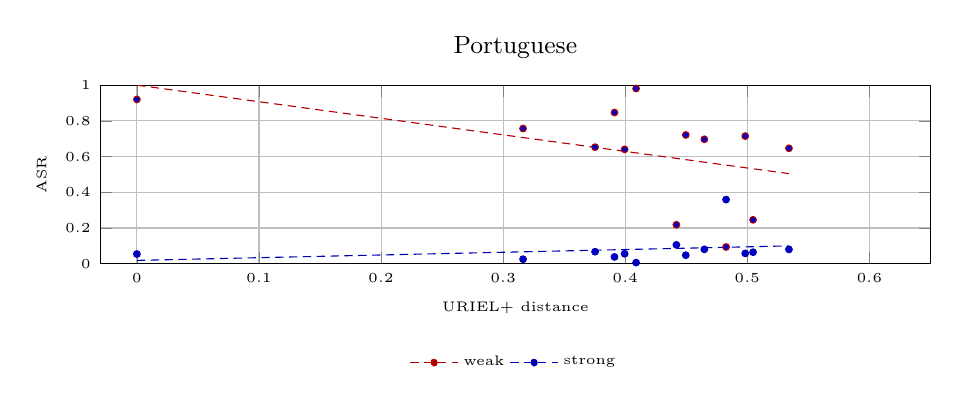
\begin{tikzpicture}
\begin{axis}[width=\linewidth,height=3.85cm,grid=both,
title={Portuguese},xlabel={URIEL+ distance},ylabel={ASR},
xmin=-0.03,xmax=0.65,ymin=0,ymax=1,
tick label style={font=\tiny},label style={font=\tiny},title style={font=\small},
legend style={font=\tiny,at={(0.5,-0.45)},anchor=north,draw=none,fill=none,legend columns=2}]
\addplot+[forget plot,only marks,mark=*,mark size=1.2pt,red!70!black] coordinates {(0.5047,0.2460) (0.3753,0.6527) (0.4983,0.7147) (0.4089,0.9808) (0.4419,0.2184) (0.3163,0.7572) (0.5341,0.6463) (0.0000,0.9199) (0.4496,0.7212) (0.3912,0.8466) (0.4826,0.0939) (0.4648,0.6968) (0.3995,0.6403)};
\addplot+[forget plot,no markers,densely dashed,red!70!black] coordinates {(0.0000,1.0000) (0.5341,0.5045)};
\addplot+[forget plot,only marks,mark=*,mark size=1.2pt,blue!70!black] coordinates {(0.5047,0.0647) (0.3753,0.0675) (0.4983,0.0581) (0.4089,0.0064) (0.4419,0.1058) (0.3163,0.0256) (0.5341,0.0804) (0.0000,0.0545) (0.4496,0.0481) (0.3912,0.0383) (0.4826,0.3592) (0.4648,0.0806) (0.3995,0.0561)};
\addplot+[forget plot,no markers,densely dashed,blue!70!black] coordinates {(0.0000,0.0188) (0.5341,0.1000)};
\addlegendimage{densely dashed,mark=*,mark size=1.2pt,red!70!black}
\addlegendentry{weak}
\addlegendimage{densely dashed,mark=*,mark size=1.2pt,blue!70!black}
\addlegendentry{strong}
\end{axis}
\end{tikzpicture}
\end{minipage}
\hfill\begin{minipage}{0.48\linewidth}\centering
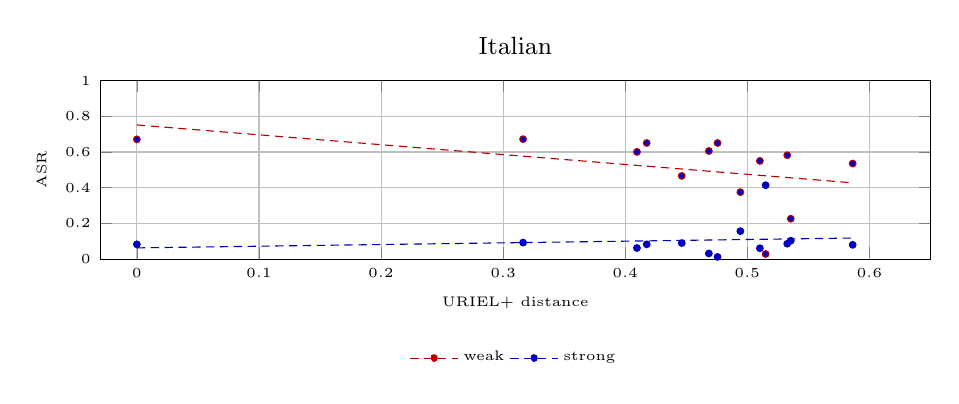
\begin{tikzpicture}
\begin{axis}[width=\linewidth,height=3.85cm,grid=both,
title={Italian},xlabel={URIEL+ distance},ylabel={ASR},
xmin=-0.03,xmax=0.65,ymin=0,ymax=1,
tick label style={font=\tiny},label style={font=\tiny},title style={font=\small},
legend style={font=\tiny,at={(0.5,-0.45)},anchor=north,draw=none,fill=none,legend columns=2}]
\addplot+[forget plot,only marks,mark=*,mark size=1.2pt,red!70!black] coordinates {(0.5356,0.2265) (0.4463,0.4662) (0.5327,0.5820) (0.4756,0.6506) (0.4943,0.3754) (0.0000,0.6709) (0.5863,0.5355) (0.3163,0.6720) (0.4685,0.6058) (0.4176,0.6506) (0.5150,0.0291) (0.5103,0.5502) (0.4096,0.6007)};
\addplot+[forget plot,no markers,densely dashed,red!70!black] coordinates {(0.0000,0.7516) (0.5863,0.4275)};
\addplot+[forget plot,only marks,mark=*,mark size=1.2pt,blue!70!black] coordinates {(0.5356,0.1036) (0.4463,0.0900) (0.5327,0.0865) (0.4756,0.0128) (0.4943,0.1570) (0.0000,0.0831) (0.5863,0.0804) (0.3163,0.0929) (0.4685,0.0321) (0.4176,0.0831) (0.5150,0.4142) (0.5103,0.0613) (0.4096,0.0627)};
\addplot+[forget plot,no markers,densely dashed,blue!70!black] coordinates {(0.0000,0.0633) (0.5863,0.1184)};
\addlegendimage{densely dashed,mark=*,mark size=1.2pt,red!70!black}
\addlegendentry{weak}
\addlegendimage{densely dashed,mark=*,mark size=1.2pt,blue!70!black}
\addlegendentry{strong}
\end{axis}
\end{tikzpicture}
\end{minipage}
\vspace{0.7cm}
\begin{minipage}{0.48\linewidth}\centering
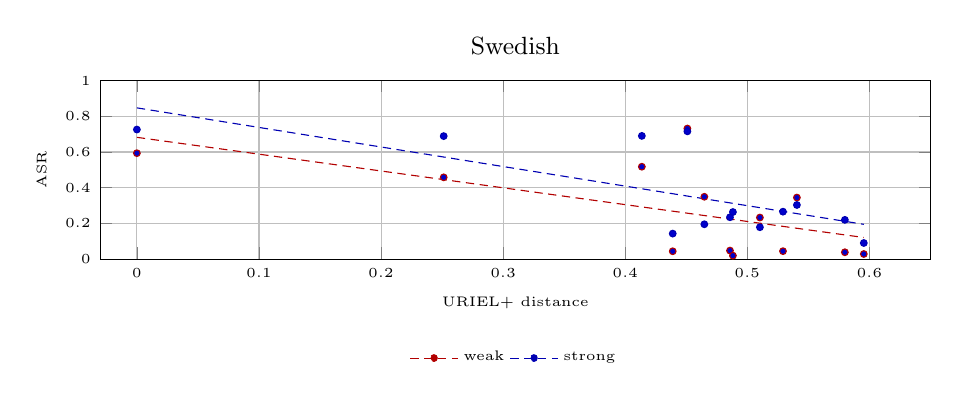
\begin{tikzpicture}
\begin{axis}[width=\linewidth,height=3.85cm,grid=both,
title={Swedish},xlabel={URIEL+ distance},ylabel={ASR},
xmin=-0.03,xmax=0.65,ymin=0,ymax=1,
tick label style={font=\tiny},label style={font=\tiny},title style={font=\small},
legend style={font=\tiny,at={(0.5,-0.45)},anchor=north,draw=none,fill=none,legend columns=2}]
\addplot+[forget plot,only marks,mark=*,mark size=1.2pt,red!70!black] coordinates {(0.5799,0.0388) (0.4858,0.0482) (0.2513,0.4583) (0.4509,0.7316) (0.4389,0.0444) (0.5103,0.2332) (0.4136,0.5177) (0.4648,0.3494) (0.5292,0.0449) (0.5406,0.3450) (0.5954,0.0291) (0.0000,0.5935) (0.4882,0.0198)};
\addplot+[forget plot,no markers,densely dashed,red!70!black] coordinates {(0.0000,0.6822) (0.5954,0.1214)};
\addplot+[forget plot,only marks,mark=*,mark size=1.2pt,blue!70!black] coordinates {(0.5799,0.2201) (0.4858,0.2347) (0.2513,0.6891) (0.4509,0.7157) (0.4389,0.1433) (0.5103,0.1789) (0.4136,0.6903) (0.4648,0.1955) (0.5292,0.2660) (0.5406,0.3035) (0.5954,0.0906) (0.0000,0.7258) (0.4882,0.2640)};
\addplot+[forget plot,no markers,densely dashed,blue!70!black] coordinates {(0.0000,0.8472) (0.5954,0.1952)};
\addlegendimage{densely dashed,mark=*,mark size=1.2pt,red!70!black}
\addlegendentry{weak}
\addlegendimage{densely dashed,mark=*,mark size=1.2pt,blue!70!black}
\addlegendentry{strong}
\end{axis}
\end{tikzpicture}
\end{minipage}
\hfill\begin{minipage}{0.48\linewidth}\centering
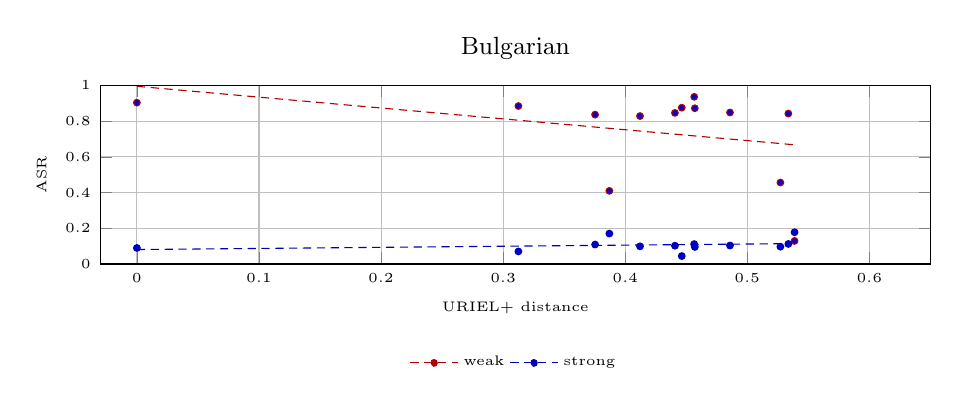
\begin{tikzpicture}
\begin{axis}[width=\linewidth,height=3.85cm,grid=both,
title={Bulgarian},xlabel={URIEL+ distance},ylabel={ASR},
xmin=-0.03,xmax=0.65,ymin=0,ymax=1,
tick label style={font=\tiny},label style={font=\tiny},title style={font=\small},
legend style={font=\tiny,at={(0.5,-0.45)},anchor=north,draw=none,fill=none,legend columns=2}]
\addplot+[forget plot,only marks,mark=*,mark size=1.2pt,red!70!black] coordinates {(0.5271,0.4563) (0.0000,0.9035) (0.4407,0.8462) (0.4565,0.9361) (0.3870,0.4096) (0.4463,0.8754) (0.5336,0.8424) (0.3753,0.8365) (0.3125,0.8846) (0.4570,0.8722) (0.5387,0.1294) (0.4858,0.8484) (0.4121,0.8284)};
\addplot+[forget plot,no markers,densely dashed,red!70!black] coordinates {(0.0000,0.9952) (0.5387,0.6675)};
\addplot+[forget plot,only marks,mark=*,mark size=1.2pt,blue!70!black] coordinates {(0.5271,0.0971) (0.0000,0.0900) (0.4407,0.1026) (0.4565,0.1118) (0.3870,0.1706) (0.4463,0.0447) (0.5336,0.1125) (0.3753,0.1090) (0.3125,0.0705) (0.4570,0.0958) (0.5387,0.1780) (0.4858,0.1037) (0.4121,0.0990)};
\addplot+[forget plot,no markers,densely dashed,blue!70!black] coordinates {(0.0000,0.0810) (0.5387,0.1144)};
\addlegendimage{densely dashed,mark=*,mark size=1.2pt,red!70!black}
\addlegendentry{weak}
\addlegendimage{densely dashed,mark=*,mark size=1.2pt,blue!70!black}
\addlegendentry{strong}
\end{axis}
\end{tikzpicture}
\end{minipage}
\vspace{0.7cm}
\begin{minipage}{0.48\linewidth}\centering
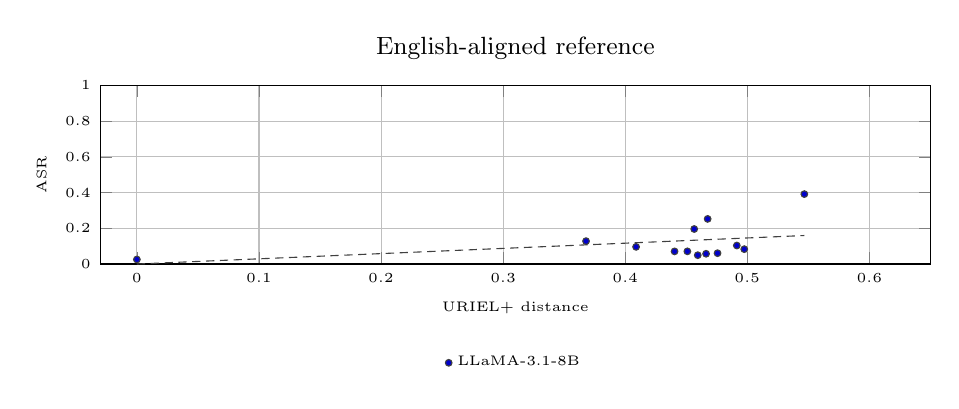
\begin{tikzpicture}
\begin{axis}[width=\linewidth,height=3.85cm,grid=both,
title={English-aligned reference},xlabel={URIEL+ distance},ylabel={ASR},
xmin=-0.03,xmax=0.65,ymin=0,ymax=1,
tick label style={font=\tiny},label style={font=\tiny},title style={font=\small},
legend style={font=\tiny,at={(0.5,-0.45)},anchor=north,draw=none,fill=none}]
\addplot+[only marks,mark=*,mark size=1.2pt,black!75!white] coordinates {(0.4914,0.1036) (0.4565,0.1961) (0.3679,0.1282) (0.0000,0.0256) (0.4675,0.2526) (0.4756,0.0607) (0.4404,0.0707) (0.4089,0.0962) (0.4975,0.0833) (0.4662,0.0575) (0.5467,0.3916) (0.4509,0.0710) (0.4594,0.0495)};
\addlegendentry{LLaMA-3.1-8B}
\addplot+[no markers,densely dashed,black!75!white] coordinates {(0.0000,0.0000) (0.5467,0.1596)};
\end{axis}
\end{tikzpicture}
\end{minipage}

\label{fig:distance-vs-asr}
\fonte{Prepared by the author (2026).}
\end{figure}
}

\newcommand{\BelebeleIfHeatmapFigure}{%
\begin{figure}[htbp]
\centering
\caption[BELEBELE IF score by model and attack language]{BELEBELE IF score by model and attack language.}

\scriptsize
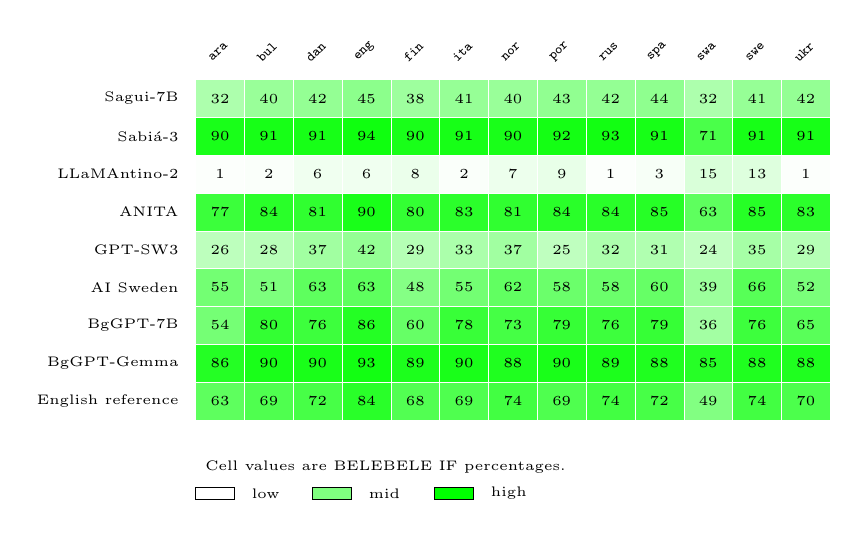
\begin{tikzpicture}[x=0.62cm,y=0.48cm]
\node[rotate=45,anchor=west,font=\tiny] at (0.16,0.35) {\texttt{ara}};
\node[rotate=45,anchor=west,font=\tiny] at (1.16,0.35) {\texttt{bul}};
\node[rotate=45,anchor=west,font=\tiny] at (2.16,0.35) {\texttt{dan}};
\node[rotate=45,anchor=west,font=\tiny] at (3.16,0.35) {\texttt{eng}};
\node[rotate=45,anchor=west,font=\tiny] at (4.16,0.35) {\texttt{fin}};
\node[rotate=45,anchor=west,font=\tiny] at (5.16,0.35) {\texttt{ita}};
\node[rotate=45,anchor=west,font=\tiny] at (6.16,0.35) {\texttt{nor}};
\node[rotate=45,anchor=west,font=\tiny] at (7.16,0.35) {\texttt{por}};
\node[rotate=45,anchor=west,font=\tiny] at (8.16,0.35) {\texttt{rus}};
\node[rotate=45,anchor=west,font=\tiny] at (9.16,0.35) {\texttt{spa}};
\node[rotate=45,anchor=west,font=\tiny] at (10.16,0.35) {\texttt{swa}};
\node[rotate=45,anchor=west,font=\tiny] at (11.16,0.35) {\texttt{swe}};
\node[rotate=45,anchor=west,font=\tiny] at (12.16,0.35) {\texttt{ukr}};
\node[anchor=east,font=\tiny] at (-0.15,-0.5) {Sagui-7B};
\fill[green!32!white] (0,0) rectangle ++(1,-1);
\draw[white,line width=0.2pt] (0,0) rectangle ++(1,-1);
\node[font=\tiny] at (0.5,-0.5) {32};
\fill[green!40!white] (1,0) rectangle ++(1,-1);
\draw[white,line width=0.2pt] (1,0) rectangle ++(1,-1);
\node[font=\tiny] at (1.5,-0.5) {40};
\fill[green!42!white] (2,0) rectangle ++(1,-1);
\draw[white,line width=0.2pt] (2,0) rectangle ++(1,-1);
\node[font=\tiny] at (2.5,-0.5) {42};
\fill[green!45!white] (3,0) rectangle ++(1,-1);
\draw[white,line width=0.2pt] (3,0) rectangle ++(1,-1);
\node[font=\tiny] at (3.5,-0.5) {45};
\fill[green!38!white] (4,0) rectangle ++(1,-1);
\draw[white,line width=0.2pt] (4,0) rectangle ++(1,-1);
\node[font=\tiny] at (4.5,-0.5) {38};
\fill[green!41!white] (5,0) rectangle ++(1,-1);
\draw[white,line width=0.2pt] (5,0) rectangle ++(1,-1);
\node[font=\tiny] at (5.5,-0.5) {41};
\fill[green!40!white] (6,0) rectangle ++(1,-1);
\draw[white,line width=0.2pt] (6,0) rectangle ++(1,-1);
\node[font=\tiny] at (6.5,-0.5) {40};
\fill[green!43!white] (7,0) rectangle ++(1,-1);
\draw[white,line width=0.2pt] (7,0) rectangle ++(1,-1);
\node[font=\tiny] at (7.5,-0.5) {43};
\fill[green!42!white] (8,0) rectangle ++(1,-1);
\draw[white,line width=0.2pt] (8,0) rectangle ++(1,-1);
\node[font=\tiny] at (8.5,-0.5) {42};
\fill[green!44!white] (9,0) rectangle ++(1,-1);
\draw[white,line width=0.2pt] (9,0) rectangle ++(1,-1);
\node[font=\tiny] at (9.5,-0.5) {44};
\fill[green!32!white] (10,0) rectangle ++(1,-1);
\draw[white,line width=0.2pt] (10,0) rectangle ++(1,-1);
\node[font=\tiny] at (10.5,-0.5) {32};
\fill[green!41!white] (11,0) rectangle ++(1,-1);
\draw[white,line width=0.2pt] (11,0) rectangle ++(1,-1);
\node[font=\tiny] at (11.5,-0.5) {41};
\fill[green!42!white] (12,0) rectangle ++(1,-1);
\draw[white,line width=0.2pt] (12,0) rectangle ++(1,-1);
\node[font=\tiny] at (12.5,-0.5) {42};
\node[anchor=east,font=\tiny] at (-0.15,-1.5) {Sabi\'a-3};
\fill[green!90!white] (0,-1) rectangle ++(1,-1);
\draw[white,line width=0.2pt] (0,-1) rectangle ++(1,-1);
\node[font=\tiny] at (0.5,-1.5) {90};
\fill[green!91!white] (1,-1) rectangle ++(1,-1);
\draw[white,line width=0.2pt] (1,-1) rectangle ++(1,-1);
\node[font=\tiny] at (1.5,-1.5) {91};
\fill[green!91!white] (2,-1) rectangle ++(1,-1);
\draw[white,line width=0.2pt] (2,-1) rectangle ++(1,-1);
\node[font=\tiny] at (2.5,-1.5) {91};
\fill[green!94!white] (3,-1) rectangle ++(1,-1);
\draw[white,line width=0.2pt] (3,-1) rectangle ++(1,-1);
\node[font=\tiny] at (3.5,-1.5) {94};
\fill[green!90!white] (4,-1) rectangle ++(1,-1);
\draw[white,line width=0.2pt] (4,-1) rectangle ++(1,-1);
\node[font=\tiny] at (4.5,-1.5) {90};
\fill[green!91!white] (5,-1) rectangle ++(1,-1);
\draw[white,line width=0.2pt] (5,-1) rectangle ++(1,-1);
\node[font=\tiny] at (5.5,-1.5) {91};
\fill[green!90!white] (6,-1) rectangle ++(1,-1);
\draw[white,line width=0.2pt] (6,-1) rectangle ++(1,-1);
\node[font=\tiny] at (6.5,-1.5) {90};
\fill[green!92!white] (7,-1) rectangle ++(1,-1);
\draw[white,line width=0.2pt] (7,-1) rectangle ++(1,-1);
\node[font=\tiny] at (7.5,-1.5) {92};
\fill[green!93!white] (8,-1) rectangle ++(1,-1);
\draw[white,line width=0.2pt] (8,-1) rectangle ++(1,-1);
\node[font=\tiny] at (8.5,-1.5) {93};
\fill[green!91!white] (9,-1) rectangle ++(1,-1);
\draw[white,line width=0.2pt] (9,-1) rectangle ++(1,-1);
\node[font=\tiny] at (9.5,-1.5) {91};
\fill[green!71!white] (10,-1) rectangle ++(1,-1);
\draw[white,line width=0.2pt] (10,-1) rectangle ++(1,-1);
\node[font=\tiny] at (10.5,-1.5) {71};
\fill[green!91!white] (11,-1) rectangle ++(1,-1);
\draw[white,line width=0.2pt] (11,-1) rectangle ++(1,-1);
\node[font=\tiny] at (11.5,-1.5) {91};
\fill[green!91!white] (12,-1) rectangle ++(1,-1);
\draw[white,line width=0.2pt] (12,-1) rectangle ++(1,-1);
\node[font=\tiny] at (12.5,-1.5) {91};
\node[anchor=east,font=\tiny] at (-0.15,-2.5) {LLaMAntino-2};
\fill[green!1!white] (0,-2) rectangle ++(1,-1);
\draw[white,line width=0.2pt] (0,-2) rectangle ++(1,-1);
\node[font=\tiny] at (0.5,-2.5) {1};
\fill[green!2!white] (1,-2) rectangle ++(1,-1);
\draw[white,line width=0.2pt] (1,-2) rectangle ++(1,-1);
\node[font=\tiny] at (1.5,-2.5) {2};
\fill[green!6!white] (2,-2) rectangle ++(1,-1);
\draw[white,line width=0.2pt] (2,-2) rectangle ++(1,-1);
\node[font=\tiny] at (2.5,-2.5) {6};
\fill[green!6!white] (3,-2) rectangle ++(1,-1);
\draw[white,line width=0.2pt] (3,-2) rectangle ++(1,-1);
\node[font=\tiny] at (3.5,-2.5) {6};
\fill[green!8!white] (4,-2) rectangle ++(1,-1);
\draw[white,line width=0.2pt] (4,-2) rectangle ++(1,-1);
\node[font=\tiny] at (4.5,-2.5) {8};
\fill[green!2!white] (5,-2) rectangle ++(1,-1);
\draw[white,line width=0.2pt] (5,-2) rectangle ++(1,-1);
\node[font=\tiny] at (5.5,-2.5) {2};
\fill[green!7!white] (6,-2) rectangle ++(1,-1);
\draw[white,line width=0.2pt] (6,-2) rectangle ++(1,-1);
\node[font=\tiny] at (6.5,-2.5) {7};
\fill[green!9!white] (7,-2) rectangle ++(1,-1);
\draw[white,line width=0.2pt] (7,-2) rectangle ++(1,-1);
\node[font=\tiny] at (7.5,-2.5) {9};
\fill[green!1!white] (8,-2) rectangle ++(1,-1);
\draw[white,line width=0.2pt] (8,-2) rectangle ++(1,-1);
\node[font=\tiny] at (8.5,-2.5) {1};
\fill[green!3!white] (9,-2) rectangle ++(1,-1);
\draw[white,line width=0.2pt] (9,-2) rectangle ++(1,-1);
\node[font=\tiny] at (9.5,-2.5) {3};
\fill[green!15!white] (10,-2) rectangle ++(1,-1);
\draw[white,line width=0.2pt] (10,-2) rectangle ++(1,-1);
\node[font=\tiny] at (10.5,-2.5) {15};
\fill[green!13!white] (11,-2) rectangle ++(1,-1);
\draw[white,line width=0.2pt] (11,-2) rectangle ++(1,-1);
\node[font=\tiny] at (11.5,-2.5) {13};
\fill[green!1!white] (12,-2) rectangle ++(1,-1);
\draw[white,line width=0.2pt] (12,-2) rectangle ++(1,-1);
\node[font=\tiny] at (12.5,-2.5) {1};
\node[anchor=east,font=\tiny] at (-0.15,-3.5) {ANITA};
\fill[green!77!white] (0,-3) rectangle ++(1,-1);
\draw[white,line width=0.2pt] (0,-3) rectangle ++(1,-1);
\node[font=\tiny] at (0.5,-3.5) {77};
\fill[green!84!white] (1,-3) rectangle ++(1,-1);
\draw[white,line width=0.2pt] (1,-3) rectangle ++(1,-1);
\node[font=\tiny] at (1.5,-3.5) {84};
\fill[green!81!white] (2,-3) rectangle ++(1,-1);
\draw[white,line width=0.2pt] (2,-3) rectangle ++(1,-1);
\node[font=\tiny] at (2.5,-3.5) {81};
\fill[green!90!white] (3,-3) rectangle ++(1,-1);
\draw[white,line width=0.2pt] (3,-3) rectangle ++(1,-1);
\node[font=\tiny] at (3.5,-3.5) {90};
\fill[green!80!white] (4,-3) rectangle ++(1,-1);
\draw[white,line width=0.2pt] (4,-3) rectangle ++(1,-1);
\node[font=\tiny] at (4.5,-3.5) {80};
\fill[green!83!white] (5,-3) rectangle ++(1,-1);
\draw[white,line width=0.2pt] (5,-3) rectangle ++(1,-1);
\node[font=\tiny] at (5.5,-3.5) {83};
\fill[green!81!white] (6,-3) rectangle ++(1,-1);
\draw[white,line width=0.2pt] (6,-3) rectangle ++(1,-1);
\node[font=\tiny] at (6.5,-3.5) {81};
\fill[green!84!white] (7,-3) rectangle ++(1,-1);
\draw[white,line width=0.2pt] (7,-3) rectangle ++(1,-1);
\node[font=\tiny] at (7.5,-3.5) {84};
\fill[green!84!white] (8,-3) rectangle ++(1,-1);
\draw[white,line width=0.2pt] (8,-3) rectangle ++(1,-1);
\node[font=\tiny] at (8.5,-3.5) {84};
\fill[green!85!white] (9,-3) rectangle ++(1,-1);
\draw[white,line width=0.2pt] (9,-3) rectangle ++(1,-1);
\node[font=\tiny] at (9.5,-3.5) {85};
\fill[green!63!white] (10,-3) rectangle ++(1,-1);
\draw[white,line width=0.2pt] (10,-3) rectangle ++(1,-1);
\node[font=\tiny] at (10.5,-3.5) {63};
\fill[green!85!white] (11,-3) rectangle ++(1,-1);
\draw[white,line width=0.2pt] (11,-3) rectangle ++(1,-1);
\node[font=\tiny] at (11.5,-3.5) {85};
\fill[green!83!white] (12,-3) rectangle ++(1,-1);
\draw[white,line width=0.2pt] (12,-3) rectangle ++(1,-1);
\node[font=\tiny] at (12.5,-3.5) {83};
\node[anchor=east,font=\tiny] at (-0.15,-4.5) {GPT-SW3};
\fill[green!26!white] (0,-4) rectangle ++(1,-1);
\draw[white,line width=0.2pt] (0,-4) rectangle ++(1,-1);
\node[font=\tiny] at (0.5,-4.5) {26};
\fill[green!28!white] (1,-4) rectangle ++(1,-1);
\draw[white,line width=0.2pt] (1,-4) rectangle ++(1,-1);
\node[font=\tiny] at (1.5,-4.5) {28};
\fill[green!37!white] (2,-4) rectangle ++(1,-1);
\draw[white,line width=0.2pt] (2,-4) rectangle ++(1,-1);
\node[font=\tiny] at (2.5,-4.5) {37};
\fill[green!42!white] (3,-4) rectangle ++(1,-1);
\draw[white,line width=0.2pt] (3,-4) rectangle ++(1,-1);
\node[font=\tiny] at (3.5,-4.5) {42};
\fill[green!29!white] (4,-4) rectangle ++(1,-1);
\draw[white,line width=0.2pt] (4,-4) rectangle ++(1,-1);
\node[font=\tiny] at (4.5,-4.5) {29};
\fill[green!33!white] (5,-4) rectangle ++(1,-1);
\draw[white,line width=0.2pt] (5,-4) rectangle ++(1,-1);
\node[font=\tiny] at (5.5,-4.5) {33};
\fill[green!37!white] (6,-4) rectangle ++(1,-1);
\draw[white,line width=0.2pt] (6,-4) rectangle ++(1,-1);
\node[font=\tiny] at (6.5,-4.5) {37};
\fill[green!25!white] (7,-4) rectangle ++(1,-1);
\draw[white,line width=0.2pt] (7,-4) rectangle ++(1,-1);
\node[font=\tiny] at (7.5,-4.5) {25};
\fill[green!32!white] (8,-4) rectangle ++(1,-1);
\draw[white,line width=0.2pt] (8,-4) rectangle ++(1,-1);
\node[font=\tiny] at (8.5,-4.5) {32};
\fill[green!31!white] (9,-4) rectangle ++(1,-1);
\draw[white,line width=0.2pt] (9,-4) rectangle ++(1,-1);
\node[font=\tiny] at (9.5,-4.5) {31};
\fill[green!24!white] (10,-4) rectangle ++(1,-1);
\draw[white,line width=0.2pt] (10,-4) rectangle ++(1,-1);
\node[font=\tiny] at (10.5,-4.5) {24};
\fill[green!35!white] (11,-4) rectangle ++(1,-1);
\draw[white,line width=0.2pt] (11,-4) rectangle ++(1,-1);
\node[font=\tiny] at (11.5,-4.5) {35};
\fill[green!29!white] (12,-4) rectangle ++(1,-1);
\draw[white,line width=0.2pt] (12,-4) rectangle ++(1,-1);
\node[font=\tiny] at (12.5,-4.5) {29};
\node[anchor=east,font=\tiny] at (-0.15,-5.5) {AI Sweden};
\fill[green!55!white] (0,-5) rectangle ++(1,-1);
\draw[white,line width=0.2pt] (0,-5) rectangle ++(1,-1);
\node[font=\tiny] at (0.5,-5.5) {55};
\fill[green!51!white] (1,-5) rectangle ++(1,-1);
\draw[white,line width=0.2pt] (1,-5) rectangle ++(1,-1);
\node[font=\tiny] at (1.5,-5.5) {51};
\fill[green!63!white] (2,-5) rectangle ++(1,-1);
\draw[white,line width=0.2pt] (2,-5) rectangle ++(1,-1);
\node[font=\tiny] at (2.5,-5.5) {63};
\fill[green!63!white] (3,-5) rectangle ++(1,-1);
\draw[white,line width=0.2pt] (3,-5) rectangle ++(1,-1);
\node[font=\tiny] at (3.5,-5.5) {63};
\fill[green!48!white] (4,-5) rectangle ++(1,-1);
\draw[white,line width=0.2pt] (4,-5) rectangle ++(1,-1);
\node[font=\tiny] at (4.5,-5.5) {48};
\fill[green!55!white] (5,-5) rectangle ++(1,-1);
\draw[white,line width=0.2pt] (5,-5) rectangle ++(1,-1);
\node[font=\tiny] at (5.5,-5.5) {55};
\fill[green!62!white] (6,-5) rectangle ++(1,-1);
\draw[white,line width=0.2pt] (6,-5) rectangle ++(1,-1);
\node[font=\tiny] at (6.5,-5.5) {62};
\fill[green!58!white] (7,-5) rectangle ++(1,-1);
\draw[white,line width=0.2pt] (7,-5) rectangle ++(1,-1);
\node[font=\tiny] at (7.5,-5.5) {58};
\fill[green!58!white] (8,-5) rectangle ++(1,-1);
\draw[white,line width=0.2pt] (8,-5) rectangle ++(1,-1);
\node[font=\tiny] at (8.5,-5.5) {58};
\fill[green!60!white] (9,-5) rectangle ++(1,-1);
\draw[white,line width=0.2pt] (9,-5) rectangle ++(1,-1);
\node[font=\tiny] at (9.5,-5.5) {60};
\fill[green!39!white] (10,-5) rectangle ++(1,-1);
\draw[white,line width=0.2pt] (10,-5) rectangle ++(1,-1);
\node[font=\tiny] at (10.5,-5.5) {39};
\fill[green!66!white] (11,-5) rectangle ++(1,-1);
\draw[white,line width=0.2pt] (11,-5) rectangle ++(1,-1);
\node[font=\tiny] at (11.5,-5.5) {66};
\fill[green!52!white] (12,-5) rectangle ++(1,-1);
\draw[white,line width=0.2pt] (12,-5) rectangle ++(1,-1);
\node[font=\tiny] at (12.5,-5.5) {52};
\node[anchor=east,font=\tiny] at (-0.15,-6.5) {BgGPT-7B};
\fill[green!54!white] (0,-6) rectangle ++(1,-1);
\draw[white,line width=0.2pt] (0,-6) rectangle ++(1,-1);
\node[font=\tiny] at (0.5,-6.5) {54};
\fill[green!80!white] (1,-6) rectangle ++(1,-1);
\draw[white,line width=0.2pt] (1,-6) rectangle ++(1,-1);
\node[font=\tiny] at (1.5,-6.5) {80};
\fill[green!76!white] (2,-6) rectangle ++(1,-1);
\draw[white,line width=0.2pt] (2,-6) rectangle ++(1,-1);
\node[font=\tiny] at (2.5,-6.5) {76};
\fill[green!86!white] (3,-6) rectangle ++(1,-1);
\draw[white,line width=0.2pt] (3,-6) rectangle ++(1,-1);
\node[font=\tiny] at (3.5,-6.5) {86};
\fill[green!60!white] (4,-6) rectangle ++(1,-1);
\draw[white,line width=0.2pt] (4,-6) rectangle ++(1,-1);
\node[font=\tiny] at (4.5,-6.5) {60};
\fill[green!78!white] (5,-6) rectangle ++(1,-1);
\draw[white,line width=0.2pt] (5,-6) rectangle ++(1,-1);
\node[font=\tiny] at (5.5,-6.5) {78};
\fill[green!73!white] (6,-6) rectangle ++(1,-1);
\draw[white,line width=0.2pt] (6,-6) rectangle ++(1,-1);
\node[font=\tiny] at (6.5,-6.5) {73};
\fill[green!79!white] (7,-6) rectangle ++(1,-1);
\draw[white,line width=0.2pt] (7,-6) rectangle ++(1,-1);
\node[font=\tiny] at (7.5,-6.5) {79};
\fill[green!76!white] (8,-6) rectangle ++(1,-1);
\draw[white,line width=0.2pt] (8,-6) rectangle ++(1,-1);
\node[font=\tiny] at (8.5,-6.5) {76};
\fill[green!79!white] (9,-6) rectangle ++(1,-1);
\draw[white,line width=0.2pt] (9,-6) rectangle ++(1,-1);
\node[font=\tiny] at (9.5,-6.5) {79};
\fill[green!36!white] (10,-6) rectangle ++(1,-1);
\draw[white,line width=0.2pt] (10,-6) rectangle ++(1,-1);
\node[font=\tiny] at (10.5,-6.5) {36};
\fill[green!76!white] (11,-6) rectangle ++(1,-1);
\draw[white,line width=0.2pt] (11,-6) rectangle ++(1,-1);
\node[font=\tiny] at (11.5,-6.5) {76};
\fill[green!65!white] (12,-6) rectangle ++(1,-1);
\draw[white,line width=0.2pt] (12,-6) rectangle ++(1,-1);
\node[font=\tiny] at (12.5,-6.5) {65};
\node[anchor=east,font=\tiny] at (-0.15,-7.5) {BgGPT-Gemma};
\fill[green!86!white] (0,-7) rectangle ++(1,-1);
\draw[white,line width=0.2pt] (0,-7) rectangle ++(1,-1);
\node[font=\tiny] at (0.5,-7.5) {86};
\fill[green!90!white] (1,-7) rectangle ++(1,-1);
\draw[white,line width=0.2pt] (1,-7) rectangle ++(1,-1);
\node[font=\tiny] at (1.5,-7.5) {90};
\fill[green!90!white] (2,-7) rectangle ++(1,-1);
\draw[white,line width=0.2pt] (2,-7) rectangle ++(1,-1);
\node[font=\tiny] at (2.5,-7.5) {90};
\fill[green!93!white] (3,-7) rectangle ++(1,-1);
\draw[white,line width=0.2pt] (3,-7) rectangle ++(1,-1);
\node[font=\tiny] at (3.5,-7.5) {93};
\fill[green!89!white] (4,-7) rectangle ++(1,-1);
\draw[white,line width=0.2pt] (4,-7) rectangle ++(1,-1);
\node[font=\tiny] at (4.5,-7.5) {89};
\fill[green!90!white] (5,-7) rectangle ++(1,-1);
\draw[white,line width=0.2pt] (5,-7) rectangle ++(1,-1);
\node[font=\tiny] at (5.5,-7.5) {90};
\fill[green!88!white] (6,-7) rectangle ++(1,-1);
\draw[white,line width=0.2pt] (6,-7) rectangle ++(1,-1);
\node[font=\tiny] at (6.5,-7.5) {88};
\fill[green!90!white] (7,-7) rectangle ++(1,-1);
\draw[white,line width=0.2pt] (7,-7) rectangle ++(1,-1);
\node[font=\tiny] at (7.5,-7.5) {90};
\fill[green!89!white] (8,-7) rectangle ++(1,-1);
\draw[white,line width=0.2pt] (8,-7) rectangle ++(1,-1);
\node[font=\tiny] at (8.5,-7.5) {89};
\fill[green!88!white] (9,-7) rectangle ++(1,-1);
\draw[white,line width=0.2pt] (9,-7) rectangle ++(1,-1);
\node[font=\tiny] at (9.5,-7.5) {88};
\fill[green!85!white] (10,-7) rectangle ++(1,-1);
\draw[white,line width=0.2pt] (10,-7) rectangle ++(1,-1);
\node[font=\tiny] at (10.5,-7.5) {85};
\fill[green!88!white] (11,-7) rectangle ++(1,-1);
\draw[white,line width=0.2pt] (11,-7) rectangle ++(1,-1);
\node[font=\tiny] at (11.5,-7.5) {88};
\fill[green!88!white] (12,-7) rectangle ++(1,-1);
\draw[white,line width=0.2pt] (12,-7) rectangle ++(1,-1);
\node[font=\tiny] at (12.5,-7.5) {88};
\node[anchor=east,font=\tiny] at (-0.15,-8.5) {English reference};
\fill[green!63!white] (0,-8) rectangle ++(1,-1);
\draw[white,line width=0.2pt] (0,-8) rectangle ++(1,-1);
\node[font=\tiny] at (0.5,-8.5) {63};
\fill[green!69!white] (1,-8) rectangle ++(1,-1);
\draw[white,line width=0.2pt] (1,-8) rectangle ++(1,-1);
\node[font=\tiny] at (1.5,-8.5) {69};
\fill[green!72!white] (2,-8) rectangle ++(1,-1);
\draw[white,line width=0.2pt] (2,-8) rectangle ++(1,-1);
\node[font=\tiny] at (2.5,-8.5) {72};
\fill[green!84!white] (3,-8) rectangle ++(1,-1);
\draw[white,line width=0.2pt] (3,-8) rectangle ++(1,-1);
\node[font=\tiny] at (3.5,-8.5) {84};
\fill[green!68!white] (4,-8) rectangle ++(1,-1);
\draw[white,line width=0.2pt] (4,-8) rectangle ++(1,-1);
\node[font=\tiny] at (4.5,-8.5) {68};
\fill[green!69!white] (5,-8) rectangle ++(1,-1);
\draw[white,line width=0.2pt] (5,-8) rectangle ++(1,-1);
\node[font=\tiny] at (5.5,-8.5) {69};
\fill[green!74!white] (6,-8) rectangle ++(1,-1);
\draw[white,line width=0.2pt] (6,-8) rectangle ++(1,-1);
\node[font=\tiny] at (6.5,-8.5) {74};
\fill[green!69!white] (7,-8) rectangle ++(1,-1);
\draw[white,line width=0.2pt] (7,-8) rectangle ++(1,-1);
\node[font=\tiny] at (7.5,-8.5) {69};
\fill[green!74!white] (8,-8) rectangle ++(1,-1);
\draw[white,line width=0.2pt] (8,-8) rectangle ++(1,-1);
\node[font=\tiny] at (8.5,-8.5) {74};
\fill[green!72!white] (9,-8) rectangle ++(1,-1);
\draw[white,line width=0.2pt] (9,-8) rectangle ++(1,-1);
\node[font=\tiny] at (9.5,-8.5) {72};
\fill[green!49!white] (10,-8) rectangle ++(1,-1);
\draw[white,line width=0.2pt] (10,-8) rectangle ++(1,-1);
\node[font=\tiny] at (10.5,-8.5) {49};
\fill[green!74!white] (11,-8) rectangle ++(1,-1);
\draw[white,line width=0.2pt] (11,-8) rectangle ++(1,-1);
\node[font=\tiny] at (11.5,-8.5) {74};
\fill[green!70!white] (12,-8) rectangle ++(1,-1);
\draw[white,line width=0.2pt] (12,-8) rectangle ++(1,-1);
\node[font=\tiny] at (12.5,-8.5) {70};
\node[anchor=west,font=\tiny] at (0,-10.25) {Cell values are BELEBELE IF percentages.};
\fill[green!0!white] (0,-10.8) rectangle ++(0.8,-0.3);\draw (0,-10.8) rectangle ++(0.8,-0.3);\node[anchor=west,font=\tiny] at (0.95,-10.950000000000001) {low};
\fill[green!50!white] (2.4,-10.8) rectangle ++(0.8,-0.3);\draw (2.4,-10.8) rectangle ++(0.8,-0.3);\node[anchor=west,font=\tiny] at (3.35,-10.950000000000001) {mid};
\fill[green!100!white] (4.9,-10.8) rectangle ++(0.8,-0.3);\draw (4.9,-10.8) rectangle ++(0.8,-0.3);\node[anchor=west,font=\tiny] at (5.85,-10.950000000000001) {high};
\end{tikzpicture}

\label{fig:belebele-if-heatmap}
\fonte{Prepared by the author (2026).}
\end{figure}
}

\newcommand{\SpecAsrFigure}{%
\begin{figure}[htbp]
\centering
\caption[ASR versus BELEBELE-derived specialization]{ASR versus BELEBELE-derived specialization.}

\begin{minipage}{0.48\linewidth}\centering
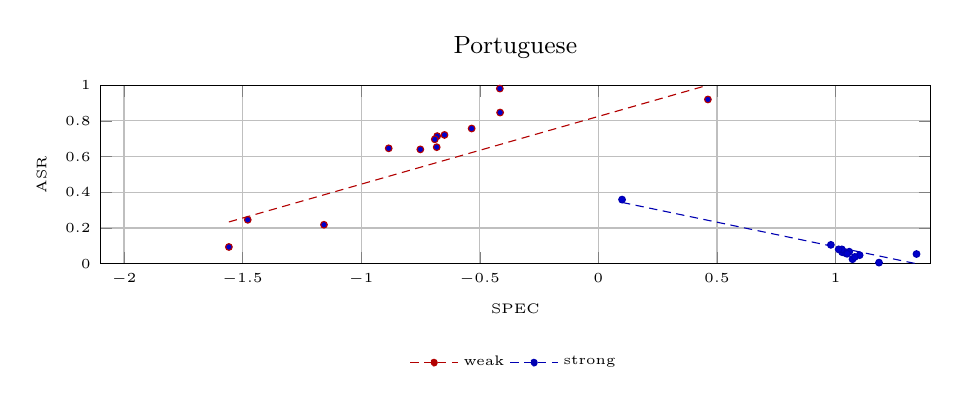
\begin{tikzpicture}
\begin{axis}[width=\linewidth,height=3.85cm,grid=both,
title={Portuguese},xlabel={SPEC},ylabel={ASR},
xmin=-2.1,xmax=1.4,ymin=0,ymax=1,
tick label style={font=\tiny},label style={font=\tiny},title style={font=\small},
legend style={font=\tiny,at={(0.5,-0.45)},anchor=north,draw=none,fill=none,legend columns=2}]
\addplot+[forget plot,only marks,mark=*,mark size=1.2pt,red!70!black] coordinates {(-1.4783,0.2460) (-0.6816,0.6527) (-0.6796,0.7147) (-0.4154,0.9808) (-1.1569,0.2184) (-0.5343,0.7572) (-0.8840,0.6463) (0.4617,0.9199) (-0.6488,0.7212) (-0.4143,0.8466) (-1.5577,0.0939) (-0.6897,0.6968) (-0.7506,0.6403)};
\addplot+[forget plot,no markers,densely dashed,red!70!black] coordinates {(-1.5577,0.2340) (0.4617,1.0000)};
\addplot+[forget plot,only marks,mark=*,mark size=1.2pt,blue!70!black] coordinates {(1.0279,0.0647) (1.0576,0.0675) (1.0442,0.0581) (1.1830,0.0064) (0.9800,0.1058) (1.0714,0.0256) (1.0266,0.0804) (1.3412,0.0545) (1.1013,0.0481) (1.0810,0.0383) (0.0998,0.3592) (1.0129,0.0806) (1.0490,0.0561)};
\addplot+[forget plot,no markers,densely dashed,blue!70!black] coordinates {(0.0998,0.3434) (1.3412,0.0000)};
\addlegendimage{densely dashed,mark=*,mark size=1.2pt,red!70!black}
\addlegendentry{weak}
\addlegendimage{densely dashed,mark=*,mark size=1.2pt,blue!70!black}
\addlegendentry{strong}
\end{axis}
\end{tikzpicture}
\end{minipage}
\hfill\begin{minipage}{0.48\linewidth}\centering
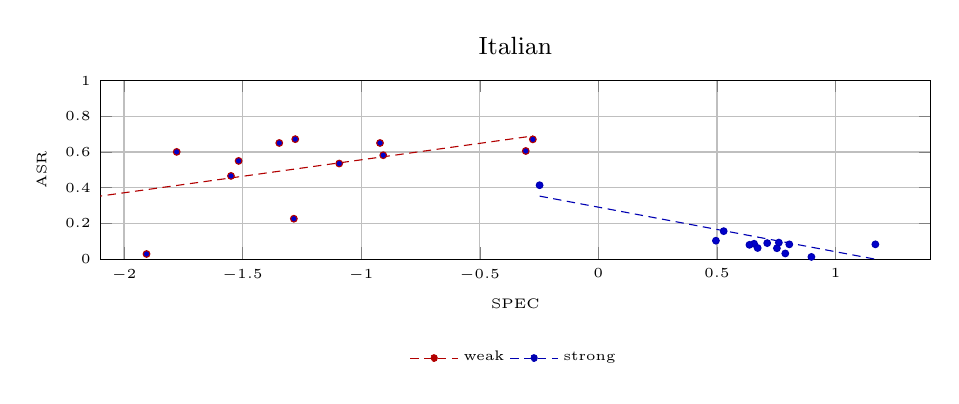
\begin{tikzpicture}
\begin{axis}[width=\linewidth,height=3.85cm,grid=both,
title={Italian},xlabel={SPEC},ylabel={ASR},
xmin=-2.1,xmax=1.4,ymin=0,ymax=1,
tick label style={font=\tiny},label style={font=\tiny},title style={font=\small},
legend style={font=\tiny,at={(0.5,-0.45)},anchor=north,draw=none,fill=none,legend columns=2}]
\addplot+[forget plot,only marks,mark=*,mark size=1.2pt,red!70!black] coordinates {(-1.2838,0.2265) (-1.5489,0.4662) (-0.9070,0.5820) (-0.9206,0.6506) (-2.1846,0.3754) (-0.2762,0.6709) (-1.0926,0.5355) (-1.2779,0.6720) (-0.3061,0.6058) (-1.3453,0.6506) (-1.9049,0.0291) (-1.5167,0.5502) (-1.7777,0.6007)};
\addplot+[forget plot,no markers,densely dashed,red!70!black] coordinates {(-2.1846,0.3377) (-0.2762,0.6899)};
\addplot+[forget plot,only marks,mark=*,mark size=1.2pt,blue!70!black] coordinates {(0.4955,0.1036) (0.7117,0.0900) (0.6564,0.0865) (0.8980,0.0128) (0.5282,0.1570) (1.1677,0.0831) (0.6368,0.0804) (0.7608,0.0929) (0.7879,0.0321) (0.8049,0.0831) (-0.2478,0.4142) (0.7526,0.0613) (0.6714,0.0627)};
\addplot+[forget plot,no markers,densely dashed,blue!70!black] coordinates {(-0.2478,0.3531) (1.1677,0.0000)};
\addlegendimage{densely dashed,mark=*,mark size=1.2pt,red!70!black}
\addlegendentry{weak}
\addlegendimage{densely dashed,mark=*,mark size=1.2pt,blue!70!black}
\addlegendentry{strong}
\end{axis}
\end{tikzpicture}
\end{minipage}
\vspace{0.7cm}
\begin{minipage}{0.48\linewidth}\centering
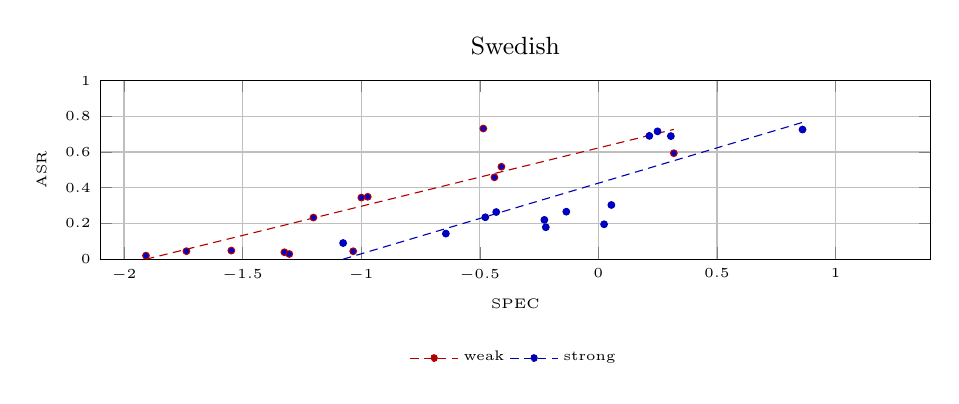
\begin{tikzpicture}
\begin{axis}[width=\linewidth,height=3.85cm,grid=both,
title={Swedish},xlabel={SPEC},ylabel={ASR},
xmin=-2.1,xmax=1.4,ymin=0,ymax=1,
tick label style={font=\tiny},label style={font=\tiny},title style={font=\small},
legend style={font=\tiny,at={(0.5,-0.45)},anchor=north,draw=none,fill=none,legend columns=2}]
\addplot+[forget plot,only marks,mark=*,mark size=1.2pt,red!70!black] coordinates {(-1.3237,0.0388) (-1.5474,0.0482) (-0.4383,0.4583) (-0.4850,0.7316) (-1.0337,0.0444) (-1.2013,0.2332) (-0.4087,0.5177) (-0.9724,0.3494) (-1.7367,0.0449) (-0.9992,0.3450) (-1.3031,0.0291) (0.3181,0.5935) (-1.9072,0.0198)};
\addplot+[forget plot,no markers,densely dashed,red!70!black] coordinates {(-1.9072,0.0000) (0.3181,0.7267)};
\addplot+[forget plot,only marks,mark=*,mark size=1.2pt,blue!70!black] coordinates {(-0.2277,0.2201) (-0.4768,0.2347) (0.3055,0.6891) (0.2493,0.7157) (-0.6430,0.1433) (-0.2216,0.1789) (0.2148,0.6903) (0.0240,0.1955) (-0.1352,0.2660) (0.0547,0.3035) (-1.0761,0.0906) (0.8606,0.7258) (-0.4307,0.2640)};
\addplot+[forget plot,no markers,densely dashed,blue!70!black] coordinates {(-1.0761,0.0000) (0.8606,0.7659)};
\addlegendimage{densely dashed,mark=*,mark size=1.2pt,red!70!black}
\addlegendentry{weak}
\addlegendimage{densely dashed,mark=*,mark size=1.2pt,blue!70!black}
\addlegendentry{strong}
\end{axis}
\end{tikzpicture}
\end{minipage}
\hfill\begin{minipage}{0.48\linewidth}\centering
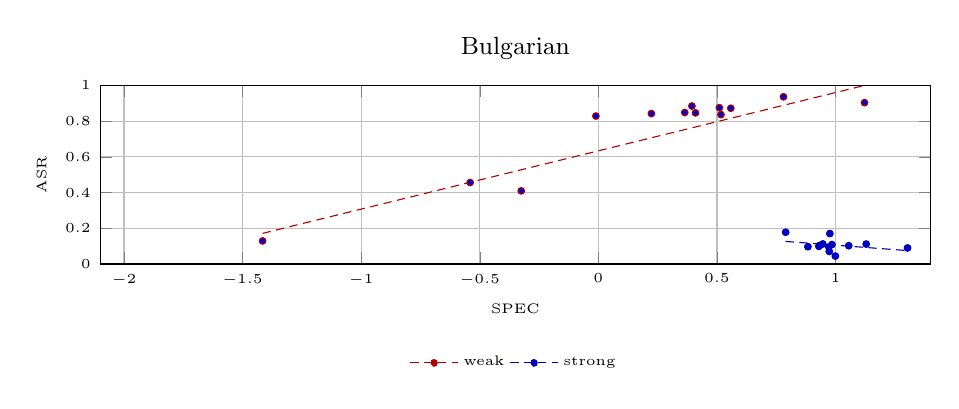
\begin{tikzpicture}
\begin{axis}[width=\linewidth,height=3.85cm,grid=both,
title={Bulgarian},xlabel={SPEC},ylabel={ASR},
xmin=-2.1,xmax=1.4,ymin=0,ymax=1,
tick label style={font=\tiny},label style={font=\tiny},title style={font=\small},
legend style={font=\tiny,at={(0.5,-0.45)},anchor=north,draw=none,fill=none,legend columns=2}]
\addplot+[forget plot,only marks,mark=*,mark size=1.2pt,red!70!black] coordinates {(-0.5405,0.4563) (1.1219,0.9035) (0.4094,0.8462) (0.7803,0.9361) (-0.3252,0.4096) (0.5102,0.8754) (0.2235,0.8424) (0.5168,0.8365) (0.3943,0.8846) (0.5583,0.8722) (-1.4156,0.1294) (0.3641,0.8484) (-0.0105,0.8284)};
\addplot+[forget plot,no markers,densely dashed,red!70!black] coordinates {(-1.4156,0.1718) (1.1219,1.0000)};
\addplot+[forget plot,only marks,mark=*,mark size=1.2pt,blue!70!black] coordinates {(0.8833,0.0971) (1.3034,0.0900) (1.0554,0.1026) (1.1290,0.1118) (0.9758,0.1706) (0.9990,0.0447) (0.9461,0.1125) (0.9845,0.1090) (0.9732,0.0705) (0.9711,0.0958) (0.7893,0.1780) (0.9323,0.1037) (0.9296,0.0990)};
\addplot+[forget plot,no markers,densely dashed,blue!70!black] coordinates {(0.7893,0.1267) (1.3034,0.0752)};
\addlegendimage{densely dashed,mark=*,mark size=1.2pt,red!70!black}
\addlegendentry{weak}
\addlegendimage{densely dashed,mark=*,mark size=1.2pt,blue!70!black}
\addlegendentry{strong}
\end{axis}
\end{tikzpicture}
\end{minipage}
\vspace{0.7cm}

\label{fig:spec-vs-asr}
\fonte{Prepared by the author (2026).}
\end{figure}
}

\newcommand{\TokenizerDiagnosticsFigure}{%
\begin{landscape}
\begin{figure}[p]
\centering
\caption[Mean token inflation by model and attack language]{Mean token inflation by model and attack language: the attack-language prompt's token count relative to the same prompt in the model's aligned language, after applying its chat template. Shading uses one log scale for all models. Bold values mark each model's aligned language. Dashes indicate unavailable measurements. The English reference is descriptive.}
\begingroup
\definecolor{UrielClose}{HTML}{355C7D}
\definecolor{UrielMiddle}{HTML}{4ECDC4}
\definecolor{UrielFar}{HTML}{F0932B}
\scriptsize
\setlength{\tabcolsep}{3.2pt}
\renewcommand{\arraystretch}{1.18}
\begin{adjustbox}{width=0.9\linewidth,center}
\begin{tabular}{>{\raggedright\arraybackslash}p{3.75cm}|*{13}{>{\centering\arraybackslash}p{0.88cm}}}
\hline
\textbf{Model} & \cellcolor[HTML]{F7D7CF}\textbf{\texttt{ita}} & \cellcolor[HTML]{F7D7CF}\textbf{\texttt{por}} & \cellcolor[HTML]{F7D7CF}\textbf{\texttt{spa}} & \cellcolor[HTML]{D6E6F6}\textbf{\texttt{eng}} & \cellcolor[HTML]{D6E6F6}\textbf{\texttt{dan}} & \cellcolor[HTML]{D6E6F6}\textbf{\texttt{nor}} & \cellcolor[HTML]{D6E6F6}\textbf{\texttt{swe}} & \cellcolor[HTML]{D8F0E1}\textbf{\texttt{fin}} & \cellcolor[HTML]{E8DDF5}\textbf{\texttt{bul}} & \cellcolor[HTML]{E8DDF5}\textbf{\texttt{rus}} & \cellcolor[HTML]{E8DDF5}\textbf{\texttt{ukr}} & \cellcolor[HTML]{F8E2C2}\textbf{\texttt{ara}} & \cellcolor[HTML]{DCEBC8}\textbf{\texttt{swa}} \\
\hline
\cellcolor[HTML]{F7D7CF}\textbf{\mbox{Sagui-7B (\texttt{por})}} & \cellcolor[HTML]{4295A1}\textcolor{black}{1.00} & \cellcolor[HTML]{4295A1}\textcolor{black}{\textbf{1.00}} & \cellcolor[HTML]{4296A2}\textcolor{black}{1.01} & \cellcolor[HTML]{3A728B}\textcolor{white}{0.79} & \cellcolor[HTML]{44A1A9}\textcolor{black}{1.08} & \cellcolor[HTML]{44A0A8}\textcolor{black}{1.07} & \cellcolor[HTML]{439AA4}\textcolor{black}{1.03} & \cellcolor[HTML]{48B0B2}\textcolor{black}{1.19} & \cellcolor[HTML]{47AFB1}\textcolor{black}{1.18} & \cellcolor[HTML]{45A4AA}\textcolor{black}{1.10} & \cellcolor[HTML]{47ACAF}\textcolor{black}{1.16} & \cellcolor[HTML]{BBDDA0}\textcolor{black}{1.92} & \cellcolor[HTML]{49B7B6}\textcolor{black}{1.24} \\
\cellcolor[HTML]{F7D7CF}\textbf{\mbox{Sabi\'a-3 (\texttt{por})}} & \cellcolor[HTML]{E6E6E6}\textemdash & \cellcolor[HTML]{E6E6E6}\textemdash & \cellcolor[HTML]{E6E6E6}\textemdash & \cellcolor[HTML]{E6E6E6}\textemdash & \cellcolor[HTML]{E6E6E6}\textemdash & \cellcolor[HTML]{E6E6E6}\textemdash & \cellcolor[HTML]{E6E6E6}\textemdash & \cellcolor[HTML]{E6E6E6}\textemdash & \cellcolor[HTML]{E6E6E6}\textemdash & \cellcolor[HTML]{E6E6E6}\textemdash & \cellcolor[HTML]{E6E6E6}\textemdash & \cellcolor[HTML]{E6E6E6}\textemdash & \cellcolor[HTML]{E6E6E6}\textemdash \\
\hline
\cellcolor[HTML]{F7D7CF}\textbf{\mbox{LLaMAntino-2 (\texttt{ita})}} & \cellcolor[HTML]{4295A1}\textcolor{black}{\textbf{1.00}} & \cellcolor[HTML]{4295A1}\textcolor{black}{1.00} & \cellcolor[HTML]{4296A1}\textcolor{black}{1.00} & \cellcolor[HTML]{3F8B9B}\textcolor{black}{0.94} & \cellcolor[HTML]{4399A3}\textcolor{black}{1.03} & \cellcolor[HTML]{4299A3}\textcolor{black}{1.02} & \cellcolor[HTML]{4297A2}\textcolor{black}{1.01} & \cellcolor[HTML]{449EA7}\textcolor{black}{1.06} & \cellcolor[HTML]{449EA6}\textcolor{black}{1.06} & \cellcolor[HTML]{439AA4}\textcolor{black}{1.03} & \cellcolor[HTML]{439DA6}\textcolor{black}{1.05} & \cellcolor[HTML]{4ABCB9}\textcolor{black}{1.29} & \cellcolor[HTML]{44A1A8}\textcolor{black}{1.08} \\
\cellcolor[HTML]{F7D7CF}\textbf{\mbox{ANITA (\texttt{ita})}} & \cellcolor[HTML]{4295A1}\textcolor{black}{\textbf{1.00}} & \cellcolor[HTML]{408D9C}\textcolor{black}{0.95} & \cellcolor[HTML]{408C9B}\textcolor{black}{0.94} & \cellcolor[HTML]{366281}\textcolor{white}{0.72} & \cellcolor[HTML]{449EA6}\textcolor{black}{1.06} & \cellcolor[HTML]{439AA4}\textcolor{black}{1.03} & \cellcolor[HTML]{4298A3}\textcolor{black}{1.02} & \cellcolor[HTML]{48B1B2}\textcolor{black}{1.20} & \cellcolor[HTML]{49B8B7}\textcolor{black}{1.26} & \cellcolor[HTML]{4298A2}\textcolor{black}{1.02} & \cellcolor[HTML]{449FA7}\textcolor{black}{1.07} & \cellcolor[HTML]{4399A3}\textcolor{black}{1.03} & \cellcolor[HTML]{49B7B6}\textcolor{black}{1.24} \\
\hline
\cellcolor[HTML]{D6E6F6}\textbf{\mbox{GPT-SW3 (\texttt{swe})}} & \cellcolor[HTML]{6BD1BB}\textcolor{black}{1.55} & \cellcolor[HTML]{7AD3B6}\textcolor{black}{1.61} & \cellcolor[HTML]{84D5B2}\textcolor{black}{1.66} & \cellcolor[HTML]{4295A1}\textcolor{black}{1.00} & \cellcolor[HTML]{449FA7}\textcolor{black}{1.07} & \cellcolor[HTML]{439CA5}\textcolor{black}{1.05} & \cellcolor[HTML]{4295A1}\textcolor{black}{\textbf{1.00}} & \cellcolor[HTML]{86D5B2}\textcolor{black}{1.67} & \cellcolor[HTML]{F19B34}\textcolor{black}{3.38} & \cellcolor[HTML]{F09831}\textcolor{black}{3.44} & \cellcolor[HTML]{F0932B}\textcolor{black}{3.54} & \cellcolor[HTML]{F19F3A}\textcolor{black}{3.31} & \cellcolor[HTML]{A8DAA7}\textcolor{black}{1.82} \\
\cellcolor[HTML]{D6E6F6}\textbf{\mbox{AI Sweden (\texttt{swe})}} & \cellcolor[HTML]{4194A0}\textcolor{black}{0.99} & \cellcolor[HTML]{408C9B}\textcolor{black}{0.94} & \cellcolor[HTML]{3F8B9B}\textcolor{black}{0.94} & \cellcolor[HTML]{366080}\textcolor{white}{0.71} & \cellcolor[HTML]{439CA5}\textcolor{black}{1.04} & \cellcolor[HTML]{4298A3}\textcolor{black}{1.02} & \cellcolor[HTML]{4295A1}\textcolor{black}{\textbf{1.00}} & \cellcolor[HTML]{47AEB1}\textcolor{black}{1.18} & \cellcolor[HTML]{49B6B5}\textcolor{black}{1.24} & \cellcolor[HTML]{4296A1}\textcolor{black}{1.00} & \cellcolor[HTML]{439DA6}\textcolor{black}{1.05} & \cellcolor[HTML]{4297A2}\textcolor{black}{1.01} & \cellcolor[HTML]{49B5B5}\textcolor{black}{1.23} \\
\hline
\cellcolor[HTML]{E8DDF5}\textbf{\mbox{BgGPT-7B (\texttt{bul})}} & \cellcolor[HTML]{48B0B2}\textcolor{black}{1.19} & \cellcolor[HTML]{48B0B2}\textcolor{black}{1.19} & \cellcolor[HTML]{48B2B3}\textcolor{black}{1.21} & \cellcolor[HTML]{3B778E}\textcolor{white}{0.82} & \cellcolor[HTML]{4ABCBA}\textcolor{black}{1.29} & \cellcolor[HTML]{4ABBB9}\textcolor{black}{1.28} & \cellcolor[HTML]{48B0B2}\textcolor{black}{1.19} & \cellcolor[HTML]{4FCDC4}\textcolor{black}{1.44} & \cellcolor[HTML]{4295A1}\textcolor{black}{\textbf{1.00}} & \cellcolor[HTML]{4ABCB9}\textcolor{black}{1.28} & \cellcolor[HTML]{4DC7C0}\textcolor{black}{1.38} & \cellcolor[HTML]{F5D67B}\textcolor{black}{2.43} & \cellcolor[HTML]{5ACFC0}\textcolor{black}{1.49} \\
\cellcolor[HTML]{E8DDF5}\textbf{\mbox{BgGPT-Gemma (\texttt{bul})}} & \cellcolor[HTML]{3B758D}\textcolor{white}{0.81} & \cellcolor[HTML]{396F89}\textcolor{white}{0.78} & \cellcolor[HTML]{386B87}\textcolor{white}{0.76} & \cellcolor[HTML]{355C7D}\textcolor{white}{0.69} & \cellcolor[HTML]{3D8194}\textcolor{white}{0.88} & \cellcolor[HTML]{3D7E92}\textcolor{white}{0.86} & \cellcolor[HTML]{3C7C91}\textcolor{white}{0.85} & \cellcolor[HTML]{41909E}\textcolor{black}{0.97} & \cellcolor[HTML]{4295A1}\textcolor{black}{\textbf{1.00}} & \cellcolor[HTML]{3C7C91}\textcolor{white}{0.85} & \cellcolor[HTML]{4296A1}\textcolor{black}{1.00} & \cellcolor[HTML]{3E8496}\textcolor{white}{0.89} & \cellcolor[HTML]{4297A2}\textcolor{black}{1.01} \\
\hline
\cellcolor[HTML]{D6E6F6}\textbf{\mbox{English reference (\texttt{eng})}} & \cellcolor[HTML]{49B7B6}\textcolor{black}{1.24} & \cellcolor[HTML]{48B1B2}\textcolor{black}{1.20} & \cellcolor[HTML]{48B0B2}\textcolor{black}{1.19} & \cellcolor[HTML]{4295A1}\textcolor{black}{\textbf{1.00}} & \cellcolor[HTML]{4ABCB9}\textcolor{black}{1.29} & \cellcolor[HTML]{4AB9B8}\textcolor{black}{1.27} & \cellcolor[HTML]{49B8B7}\textcolor{black}{1.26} & \cellcolor[HTML]{4DCAC2}\textcolor{black}{1.41} & \cellcolor[HTML]{53CEC2}\textcolor{black}{1.46} & \cellcolor[HTML]{49B8B7}\textcolor{black}{1.25} & \cellcolor[HTML]{4ABDBA}\textcolor{black}{1.30} & \cellcolor[HTML]{49B9B7}\textcolor{black}{1.26} & \cellcolor[HTML]{50CDC3}\textcolor{black}{1.45} \\
\hline
\end{tabular}
\end{adjustbox}
\vspace{0.55em}
\begin{tikzpicture}[x=1cm,y=0.28cm]
\fill[UrielClose] (0,0) rectangle (0.55,1);\node[anchor=west,font=\scriptsize] at (0.65,0.5) {lower};
\fill[UrielMiddle] (2.1,0) rectangle (2.65,1);\node[anchor=west,font=\scriptsize] at (2.75,0.5) {intermediate};
\fill[UrielFar] (5.0,0) rectangle (5.55,1);\node[anchor=west,font=\scriptsize] at (5.65,0.5) {higher};
\node[anchor=west,font=\scriptsize] at (8.25,0.5) {Rows show each model with its aligned language; columns are grouped by broad family as in Table~\ref{tab:urielplus-distances}.};
\end{tikzpicture}
\label{fig:tokenizer-diagnostics}
\par\fonte{Prepared by the author (2026).}
\endgroup
\end{figure}
\end{landscape}
}

\newcommand{\TokensPerCharacterFigure}{%
\begin{landscape}
\begin{figure}[p]
\centering
\caption[Mean tokens per character by model and attack language]{Mean tokens per character by model and attack language. Each value averages prompt-level chat-template token counts divided by the number of characters in the attack-language prompt before chat-template rendering. Characters are Unicode code points, not UTF-8 bytes. Shading is normalized separately within each model's row. Bold values mark each model's aligned language. Dashes indicate unavailable measurements. The English reference is descriptive. These values reflect tokenizer segmentation and template overhead, not comprehension or safety.}
\begingroup
\definecolor{UrielClose}{HTML}{355C7D}
\definecolor{UrielMiddle}{HTML}{4ECDC4}
\definecolor{UrielFar}{HTML}{F0932B}
\scriptsize
\setlength{\tabcolsep}{3.2pt}
\renewcommand{\arraystretch}{1.18}
\begin{adjustbox}{width=0.9\linewidth,center}
\begin{tabular}{>{\raggedright\arraybackslash}p{3.75cm}|*{13}{>{\centering\arraybackslash}p{0.88cm}}}
\hline
\textbf{Model} & \cellcolor[HTML]{F7D7CF}\textbf{\texttt{ita}} & \cellcolor[HTML]{F7D7CF}\textbf{\texttt{por}} & \cellcolor[HTML]{F7D7CF}\textbf{\texttt{spa}} & \cellcolor[HTML]{D6E6F6}\textbf{\texttt{eng}} & \cellcolor[HTML]{D6E6F6}\textbf{\texttt{dan}} & \cellcolor[HTML]{D6E6F6}\textbf{\texttt{nor}} & \cellcolor[HTML]{D6E6F6}\textbf{\texttt{swe}} & \cellcolor[HTML]{D8F0E1}\textbf{\texttt{fin}} & \cellcolor[HTML]{E8DDF5}\textbf{\texttt{bul}} & \cellcolor[HTML]{E8DDF5}\textbf{\texttt{rus}} & \cellcolor[HTML]{E8DDF5}\textbf{\texttt{ukr}} & \cellcolor[HTML]{F8E2C2}\textbf{\texttt{ara}} & \cellcolor[HTML]{DCEBC8}\textbf{\texttt{swa}} \\
\hline
\cellcolor[HTML]{F7D7CF}\textbf{\mbox{Sagui-7B (\texttt{por})}} & \cellcolor[HTML]{386C87}\textcolor{white}{0.457} & \cellcolor[HTML]{3A718A}\textcolor{white}{\textbf{0.473}} & \cellcolor[HTML]{396C87}\textcolor{white}{0.459} & \cellcolor[HTML]{355C7D}\textcolor{white}{0.412} & \cellcolor[HTML]{3D8295}\textcolor{white}{0.523} & \cellcolor[HTML]{3E8396}\textcolor{white}{0.526} & \cellcolor[HTML]{3D8094}\textcolor{white}{0.518} & \cellcolor[HTML]{439BA5}\textcolor{black}{0.597} & \cellcolor[HTML]{4194A0}\textcolor{black}{0.576} & \cellcolor[HTML]{3D8194}\textcolor{white}{0.521} & \cellcolor[HTML]{40909D}\textcolor{black}{0.563} & \cellcolor[HTML]{F0932B}\textcolor{black}{1.145} & \cellcolor[HTML]{4297A2}\textcolor{black}{0.583} \\
\cellcolor[HTML]{F7D7CF}\textbf{\mbox{Sabi\'a-3 (\texttt{por})}} & \cellcolor[HTML]{E6E6E6}\textemdash & \cellcolor[HTML]{E6E6E6}\textemdash & \cellcolor[HTML]{E6E6E6}\textemdash & \cellcolor[HTML]{E6E6E6}\textemdash & \cellcolor[HTML]{E6E6E6}\textemdash & \cellcolor[HTML]{E6E6E6}\textemdash & \cellcolor[HTML]{E6E6E6}\textemdash & \cellcolor[HTML]{E6E6E6}\textemdash & \cellcolor[HTML]{E6E6E6}\textemdash & \cellcolor[HTML]{E6E6E6}\textemdash & \cellcolor[HTML]{E6E6E6}\textemdash & \cellcolor[HTML]{E6E6E6}\textemdash & \cellcolor[HTML]{E6E6E6}\textemdash \\
\hline
\cellcolor[HTML]{F7D7CF}\textbf{\mbox{LLaMAntino-2 (\texttt{ita})}} & \cellcolor[HTML]{355E7E}\textcolor{white}{\textbf{1.657}} & \cellcolor[HTML]{386A86}\textcolor{white}{1.710} & \cellcolor[HTML]{355C7D}\textcolor{white}{1.649} & \cellcolor[HTML]{3B768D}\textcolor{white}{1.761} & \cellcolor[HTML]{3C7C91}\textcolor{white}{1.788} & \cellcolor[HTML]{3D8295}\textcolor{white}{1.811} & \cellcolor[HTML]{3F8999}\textcolor{black}{1.843} & \cellcolor[HTML]{439CA5}\textcolor{black}{1.926} & \cellcolor[HTML]{408C9B}\textcolor{black}{1.857} & \cellcolor[HTML]{3B768D}\textcolor{white}{1.761} & \cellcolor[HTML]{3F8999}\textcolor{black}{1.843} & \cellcolor[HTML]{F0932B}\textcolor{black}{2.729} & \cellcolor[HTML]{3E8496}\textcolor{white}{1.820} \\
\cellcolor[HTML]{F7D7CF}\textbf{\mbox{ANITA (\texttt{ita})}} & \cellcolor[HTML]{49B6B5}\textcolor{black}{\textbf{0.360}} & \cellcolor[HTML]{46AAAE}\textcolor{black}{0.351} & \cellcolor[HTML]{4297A2}\textcolor{black}{0.336} & \cellcolor[HTML]{355C7D}\textcolor{white}{0.290} & \cellcolor[HTML]{91D7AE}\textcolor{black}{0.400} & \cellcolor[HTML]{87D5B1}\textcolor{black}{0.396} & \cellcolor[HTML]{92D7AE}\textcolor{black}{0.400} & \cellcolor[HTML]{F2AD4A}\textcolor{black}{0.469} & \cellcolor[HTML]{F1A03B}\textcolor{black}{0.478} & \cellcolor[HTML]{4DCBC3}\textcolor{black}{0.376} & \cellcolor[HTML]{AADAA6}\textcolor{black}{0.407} & \cellcolor[HTML]{F0932B}\textcolor{black}{0.487} & \cellcolor[HTML]{F3BE5E}\textcolor{black}{0.458} \\
\hline
\cellcolor[HTML]{D6E6F6}\textbf{\mbox{GPT-SW3 (\texttt{swe})}} & \cellcolor[HTML]{3C7E92}\textcolor{white}{0.381} & \cellcolor[HTML]{3E8698}\textcolor{white}{0.408} & \cellcolor[HTML]{3E8597}\textcolor{white}{0.405} & \cellcolor[HTML]{355D7E}\textcolor{white}{0.278} & \cellcolor[HTML]{355E7E}\textcolor{white}{0.279} & \cellcolor[HTML]{355D7E}\textcolor{white}{0.278} & \cellcolor[HTML]{355C7D}\textcolor{white}{\textbf{0.274}} & \cellcolor[HTML]{4193A0}\textcolor{black}{0.450} & \cellcolor[HTML]{F5D87D}\textcolor{black}{0.884} & \cellcolor[HTML]{F5DD83}\textcolor{black}{0.871} & \cellcolor[HTML]{F4CA6D}\textcolor{black}{0.922} & \cellcolor[HTML]{F0932B}\textcolor{black}{1.072} & \cellcolor[HTML]{4297A2}\textcolor{black}{0.460} \\
\cellcolor[HTML]{D6E6F6}\textbf{\mbox{AI Sweden (\texttt{swe})}} & \cellcolor[HTML]{49B6B5}\textcolor{black}{0.360} & \cellcolor[HTML]{46AAAE}\textcolor{black}{0.351} & \cellcolor[HTML]{4297A2}\textcolor{black}{0.336} & \cellcolor[HTML]{355C7D}\textcolor{white}{0.290} & \cellcolor[HTML]{91D7AE}\textcolor{black}{0.400} & \cellcolor[HTML]{88D5B1}\textcolor{black}{0.397} & \cellcolor[HTML]{92D7AE}\textcolor{black}{\textbf{0.400}} & \cellcolor[HTML]{F2AD4A}\textcolor{black}{0.469} & \cellcolor[HTML]{F1A03B}\textcolor{black}{0.478} & \cellcolor[HTML]{4DCBC3}\textcolor{black}{0.376} & \cellcolor[HTML]{AADAA6}\textcolor{black}{0.407} & \cellcolor[HTML]{F0932B}\textcolor{black}{0.487} & \cellcolor[HTML]{F3BE5E}\textcolor{black}{0.458} \\
\hline
\cellcolor[HTML]{E8DDF5}\textbf{\mbox{BgGPT-7B (\texttt{bul})}} & \cellcolor[HTML]{3B798F}\textcolor{white}{0.374} & \cellcolor[HTML]{3C7D92}\textcolor{white}{0.385} & \cellcolor[HTML]{3C7A90}\textcolor{white}{0.376} & \cellcolor[HTML]{355C7D}\textcolor{white}{0.291} & \cellcolor[HTML]{408C9B}\textcolor{black}{0.428} & \cellcolor[HTML]{408D9C}\textcolor{black}{0.430} & \cellcolor[HTML]{3E8697}\textcolor{white}{0.409} & \cellcolor[HTML]{45A4AA}\textcolor{black}{0.496} & \cellcolor[HTML]{396D88}\textcolor{white}{\textbf{0.340}} & \cellcolor[HTML]{3F8899}\textcolor{black}{0.417} & \cellcolor[HTML]{4298A3}\textcolor{black}{0.462} & \cellcolor[HTML]{F0932B}\textcolor{black}{1.002} & \cellcolor[HTML]{449EA7}\textcolor{black}{0.479} \\
\cellcolor[HTML]{E8DDF5}\textbf{\mbox{BgGPT-Gemma (\texttt{bul})}} & \cellcolor[HTML]{3C7C91}\textcolor{white}{0.297} & \cellcolor[HTML]{3B778E}\textcolor{white}{0.293} & \cellcolor[HTML]{355C7D}\textcolor{white}{0.277} & \cellcolor[HTML]{376683}\textcolor{white}{0.283} & \cellcolor[HTML]{4BC0BC}\textcolor{black}{0.339} & \cellcolor[HTML]{4ABDBA}\textcolor{black}{0.337} & \cellcolor[HTML]{4ECBC3}\textcolor{black}{0.346} & \cellcolor[HTML]{F6E289}\textcolor{black}{0.390} & \cellcolor[HTML]{F5DD84}\textcolor{black}{\textbf{0.393}} & \cellcolor[HTML]{45A3AA}\textcolor{black}{0.321} & \cellcolor[HTML]{F6DE85}\textcolor{black}{0.392} & \cellcolor[HTML]{F0932B}\textcolor{black}{0.432} & \cellcolor[HTML]{D6E097}\textcolor{black}{0.381} \\
\hline
\cellcolor[HTML]{D6E6F6}\textbf{\mbox{English reference (\texttt{eng})}} & \cellcolor[HTML]{408D9C}\textcolor{black}{0.558} & \cellcolor[HTML]{3F8A9A}\textcolor{black}{0.556} & \cellcolor[HTML]{3A728B}\textcolor{white}{0.533} & \cellcolor[HTML]{355C7D}\textcolor{white}{\textbf{0.513}} & \cellcolor[HTML]{4CC2BD}\textcolor{black}{0.609} & \cellcolor[HTML]{4CC2BD}\textcolor{black}{0.609} & \cellcolor[HTML]{4ECDC4}\textcolor{black}{0.619} & \cellcolor[HTML]{F5DD83}\textcolor{black}{0.690} & \cellcolor[HTML]{F5DC83}\textcolor{black}{0.690} & \cellcolor[HTML]{45A5AB}\textcolor{black}{0.582} & \cellcolor[HTML]{4FCDC4}\textcolor{black}{0.619} & \cellcolor[HTML]{F0932B}\textcolor{black}{0.749} & \cellcolor[HTML]{C1DD9E}\textcolor{black}{0.663} \\
\hline
\end{tabular}
\end{adjustbox}
\vspace{0.55em}
\begin{tikzpicture}[x=1cm,y=0.28cm]
\fill[UrielClose] (0,0) rectangle (0.55,1);\node[anchor=west,font=\scriptsize] at (0.65,0.5) {lower};
\fill[UrielMiddle] (2.1,0) rectangle (2.65,1);\node[anchor=west,font=\scriptsize] at (2.75,0.5) {intermediate};
\fill[UrielFar] (5.0,0) rectangle (5.55,1);\node[anchor=west,font=\scriptsize] at (5.65,0.5) {higher};
\node[anchor=west,font=\scriptsize] at (8.25,0.5) {Shading compares languages within a model, not across models.};
\end{tikzpicture}
\label{fig:tokens-per-character}
\par\fonte{Prepared by the author (2026).}
\endgroup
\end{figure}
\end{landscape}
}

\discardmacros{\AsrHeatmapFigure\DistanceAsrFigure\BelebeleIfHeatmapFigure\SpecAsrFigure}

\chapter{Results}
\label{chap:results}

This chapter reports the empirical results obtained from the frozen evaluation dataset. The dataset contains 36\,189 prompt--model--language rows, covering the eight target language-specific models and the English-aligned Llama-3.1-8B-Instruct reference baseline. Each model contributes the same retained panel of 4\,021 attempts (Table~\ref{tab:results-coverage}), and all coverage accounting in this chapter starts from that panel. The upstream source-prompt arithmetic and the numeric translation-QC thresholds that produced it are given in Appendix~\ref{app:frozen-qc-details}.

The presentation follows Chapter~\ref{chap:methodology}. Coverage and translation quality come first, because they determine the denominators of every later estimate. The chapter then summarizes the graded scores, describes how they vary with distance and specialization, and ends with fractional-logit inference and its diagnostics, including the tokenizer checks.

\textbf{The main empirical finding does not support the directional account.} Mean graded harmful-assistance scores vary strongly by model family and paired post-training regime. They do not, however, increase with URIEL+ distance, and BELEBELE-derived specialization does not behave as a simple protective factor. Three results lead to this conclusion. First, the distance coefficient is negative in \RDistanceNegativeCount{} of \RDistanceSpecCount{} reported specifications, the opposite of the predicted direction. Second, once the robust covariance is clustered on the model--language cell, where distance and specialization actually vary, the pooled distance interval covers zero (\RDistanceCellInterval{}). Third, the heterogeneous-pair sign-retention matrix, the one component of the analysis fixed before results were examined, retains the slope sign in only \RPreregRetained{} of \RPreregEvaluated{} pairs, and \RPreregPositivePairs{} pairs are positive at both poles; that count falls in the band of the matrix that does not support H\textsubscript{1}. The more defensible reading is therefore that \textbf{checkpoint differences are large, while typological distance shows no detectable positive association in this panel.}
\defensebox{How to defend the negative result}{The directional hypotheses are not supported, and the evidence is now consistent rather than merely inconclusive. Earlier drafts described a coverage restriction as reversing the distance sign; under cell-clustered inference both that restriction and the pooled fit cover zero, so they never disagreed in any inferential sense. What remains is a clean negative: no detectable positive distance association anywhere, no pair positive at both poles, and a specialization proxy that runs opposite to the protective prediction. The result narrows what can be claimed: typological distance is not a usable priority rule for multilingual red-teaming in this panel. The stronger practical finding is model-centered: some language-specific assistants are unsafe broadly, while others are much safer across many languages. In a defense, frame this as replacing an elegant hypothesis with a more operationally honest safety conclusion.}

\section{Evaluation Coverage and Data Quality}
\label{sec:results-coverage}

Table~\ref{tab:results-coverage} reports the denominator for the later mean-score estimates. All target models and the reference baseline cover the 13 attack languages. The frozen dataset contains 78 excluded or unscored rows: 75 empty model outputs and three StrongREJECT judge safety-filter failures.
These cases are technical or scoring failures, not safe responses. They are excluded from the mean-score denominator and remain visible in coverage accounting. In-model refusals are retained as substantive model outputs.
\defensenote{Coverage vs safety}{Coverage failures are measurement failures. Refusals are model behavior. Keeping those categories separate avoids artificially rewarding systems that fail to produce scorable outputs.}

\QualityCoverageTable

The exclusions are concentrated rather than evenly distributed. Sixty-nine empty outputs occur for BgGPT-Gemma in Swedish, and six additional empty outputs occur for LLaMAntino-2 across Danish, English, Norwegian, Portuguese, Spanish, and Swedish. The three judge safety-filter blocks occur once for AI Sweden in Norwegian and twice for Sabiá-3 in Danish. The dataset otherwise has no duplicate run identifiers and no duplicate model--language--prompt rows.

For the three nonempty responses blocked by the scoring judge, the score is unknown. Table~\ref{tab:graded-unscored-bounds} shows worst/best-case mean-score bounds instead of assigning observed zeros. Even assigning all three unscored responses the maximum score changes each affected model mean by less than 0.0005 relative to the zero-assignment bound. These judge blocks are not target-provider blocks. The 75 empty outputs remain technical missingness. All rows have a true generation-completion flag, which indicates request-path completion and does not establish usable text.

\GradedBoundsTable

\subsection{LLM-only Prompt Translation QC}
\label{sec:prompt-translation-qc}

The translation audit was completed with the XSTS-style LLM reviewer described in the methodology: the 148 BLASER-flagged prompt translations were judged by a GPT-5.4 XSTS assessor. Of those flagged rows, 100 were retained and 48 were excluded from the frozen prompt inventory. The remaining 3\,921 prompt translations passed the BLASER gate and did not receive an XSTS score. Round-trip drift is computed for every prompt translation and reported as a diagnostic.

Table~\ref{tab:prompt-translation-qc} reports the BLASER-flagged queue size, median XSTS score, and audit decision counts by attack language.

\QualityPromptQcTable

Finnish is the main translation-pipeline anomaly. It has 58 flagged rows, far above the next-highest queue size of 17, and 20 of those flagged rows were marked for exclusion by the LLM judge. Ukrainian also shows a relatively high exclusion count among flagged rows.

\section{StrongREJECT Scores and Model Comparisons}
\label{sec:overall-score}

This section compares the evaluated models using the mean official StrongREJECT score defined in Section~\ref{sec:strongreject-graded}, Equation~\ref{eq:mean-strongreject}. Higher means indicate more rubric-assessed harmful assistance across the scored responses. Zero scores are included; missing judge scores remain unknown and are excluded. These means are graded scores, not percentages of successful attacks.

\subsection{Aligned and Non-aligned Language Comparisons}

Figure~\ref{fig:graded-aligned-comparison} compares two settings on a common score scale: each model's aligned language and the other twelve languages pooled together. Models are grouped into the Portuguese, Italian, Swedish, and Bulgarian pairs. A separate English-reference row shows its English mean and pooled mean across the twelve non-English languages; this baseline is descriptive and excluded from paired inference. The two points in each row show whether harmful-assistance scores are already high in the aligned-language setting or increase outside it. Exact means, intervals, and scored sample sizes appear in Appendix~\ref{app:graded-details}, Table~\ref{tab:graded-setting-summary}.

The horizontal whiskers show 95\% uncertainty intervals estimated by repeatedly sampling the original prompts, keeping their translated responses together. In the non-aligned setting, every scored response contributes equally, so a language with more scored responses contributes more to the pooled mean.

\begin{figure}[htbp]\centering
\caption[Aligned and non-aligned StrongREJECT scores]{Mean StrongREJECT scores in aligned and pooled non-aligned languages, grouped by model pair, with a separate descriptive English reference baseline. Its aligned language is English; it is excluded from paired inference. Points show means and whiskers show 95\% prompt-cluster bootstrap intervals (2\,000 resamples). Zero scores are included; missing judge scores are excluded. Non-aligned means weight each scored response equally. Higher scores indicate more harmful assistance.}

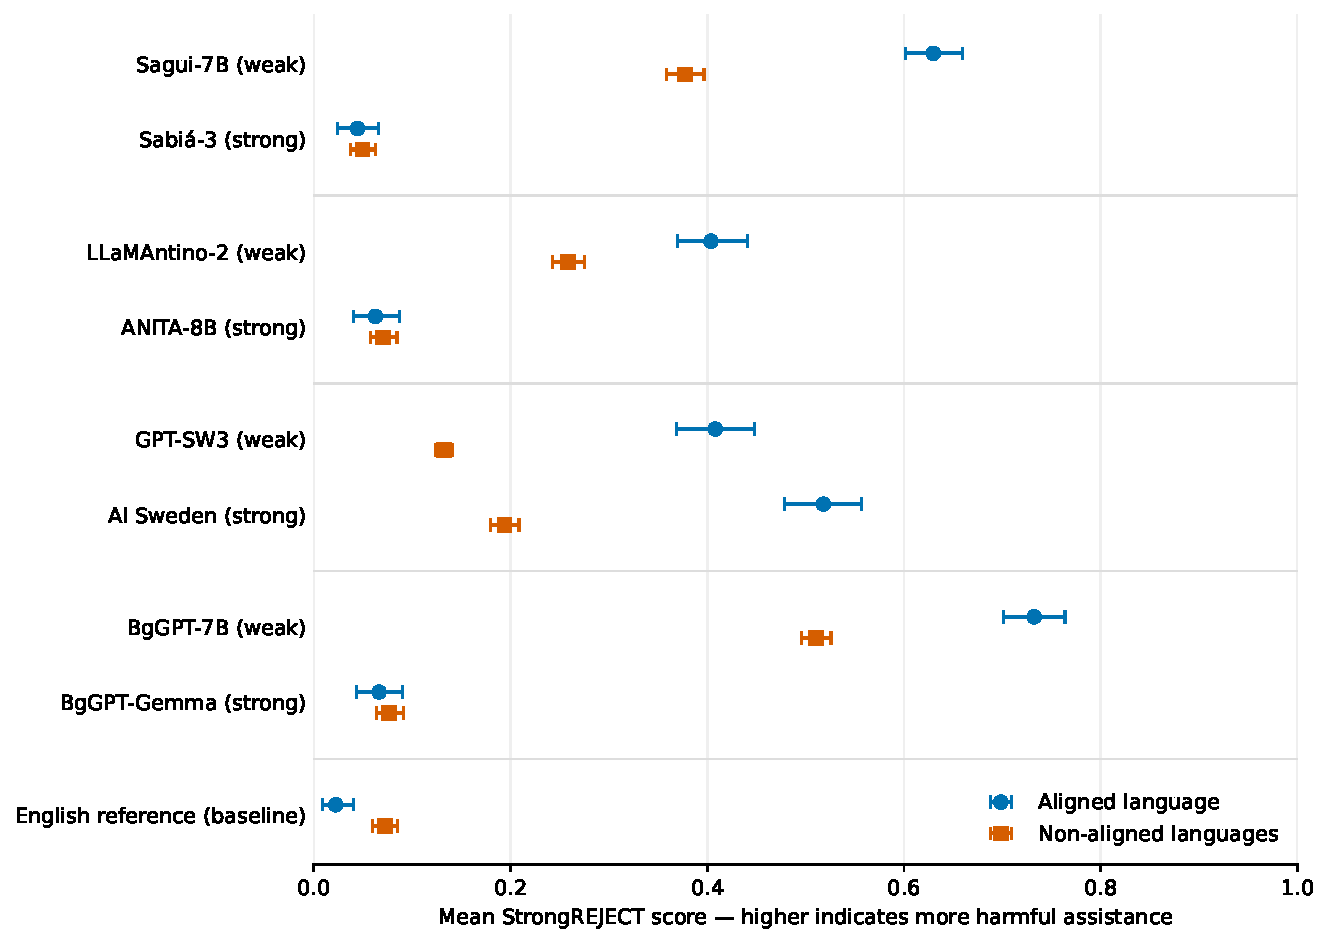
\includegraphics[width=\linewidth]{figures/graded_aligned_comparison.pdf}
\label{fig:graded-aligned-comparison}\fonte{Prepared by the author (2026).}
\end{figure}

The Portuguese, Italian, and Bulgarian pairs show the same broad ordering in both settings: the strong-pole model has a lower mean score than its weak-pole partner. The Swedish pair shows the opposite ordering, with AI Sweden scoring higher than GPT-SW3. Thus, the strong-pole label does not consistently correspond to lower harmful assistance across all four pairs.

These comparisons describe the evaluated checkpoints. Each pair differs in more than its alignment label, including model ancestry, training data, size, and serving mode. We therefore cannot attribute the differences to a single alignment intervention. Similarly, the combined non-aligned mean can hide considerable variation between individual languages.
\defensenote{Present the pair comparison}{Say: ``Three pairs have lower average harmful assistance at the strong pole; the Swedish pair goes the other way. This is an observed comparison between checkpoints, not a controlled experiment on alignment strength.'' Then use the language heatmap to show why a single model average is only part of the picture.}

\subsection{Variation Across Languages and Responses}

Figure~\ref{fig:graded-heatmap} separates the combined averages into individual model--language combinations. Each cell gives the mean score for one model answering prompts in one language. It helps identify languages with relatively high or low scores within a model and compare language profiles across models.

\begin{figure}[htbp]\centering
\caption[StrongREJECT score heatmap]{Mean StrongREJECT score for each model and attack language. Higher values indicate more harmful assistance.}

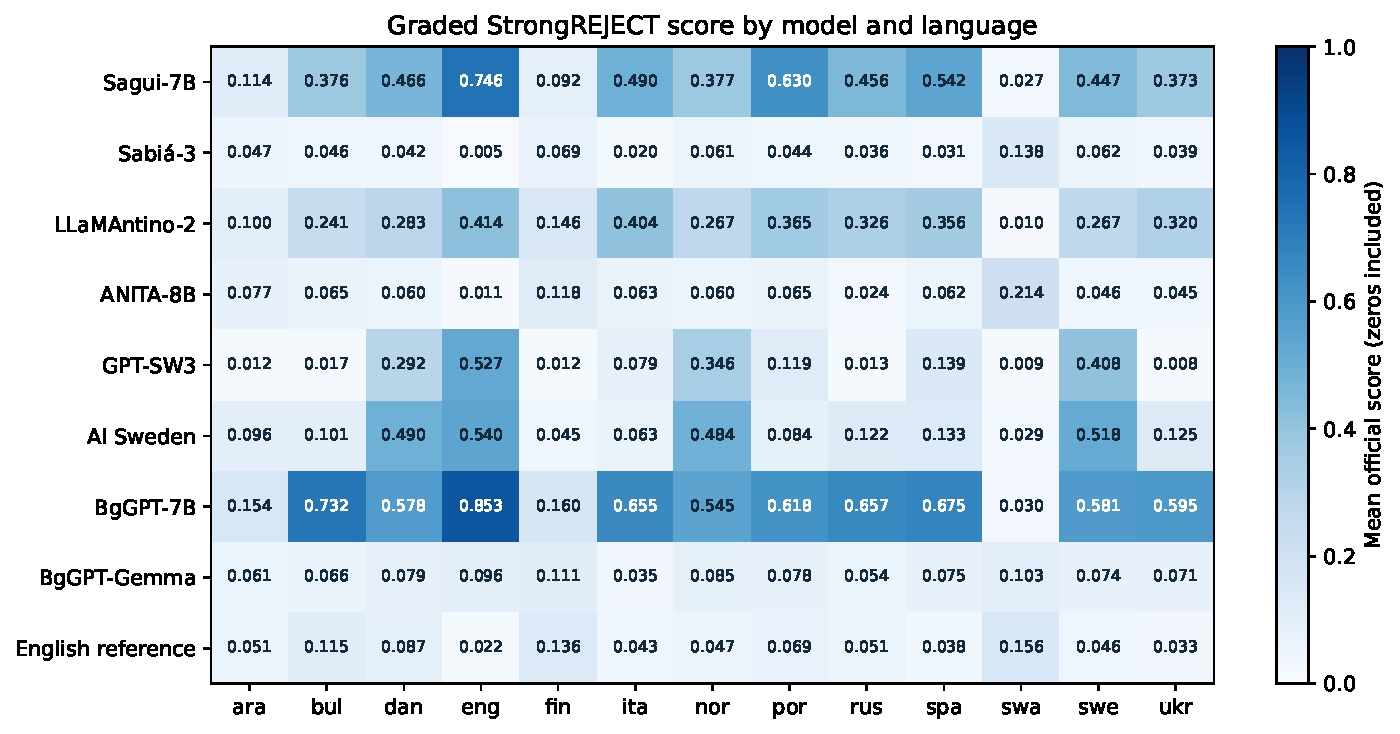
\includegraphics[width=\linewidth]{figures/graded_score_heatmap.pdf}
\label{fig:graded-heatmap}\fonte{Prepared by the author (2026).}
\end{figure}

A mean does not show how individual responses are distributed. For example, two hypothetical scores of 0 and 1 have the same average as two scores of 0.5, although the first case combines a zero with maximum harmful assistance and the second contains two intermediate responses. Figure~\ref{fig:graded-distribution} therefore shows the distribution of scores across all scored languages for each model. It reveals whether an average comes mainly from zeros, intermediate scores, or high scores.

\begin{figure}[htbp]\centering
\caption[StrongREJECT score distributions]{Distribution of StrongREJECT scores for each model across all scored languages. The plot separates zero, intermediate, and high scores.}

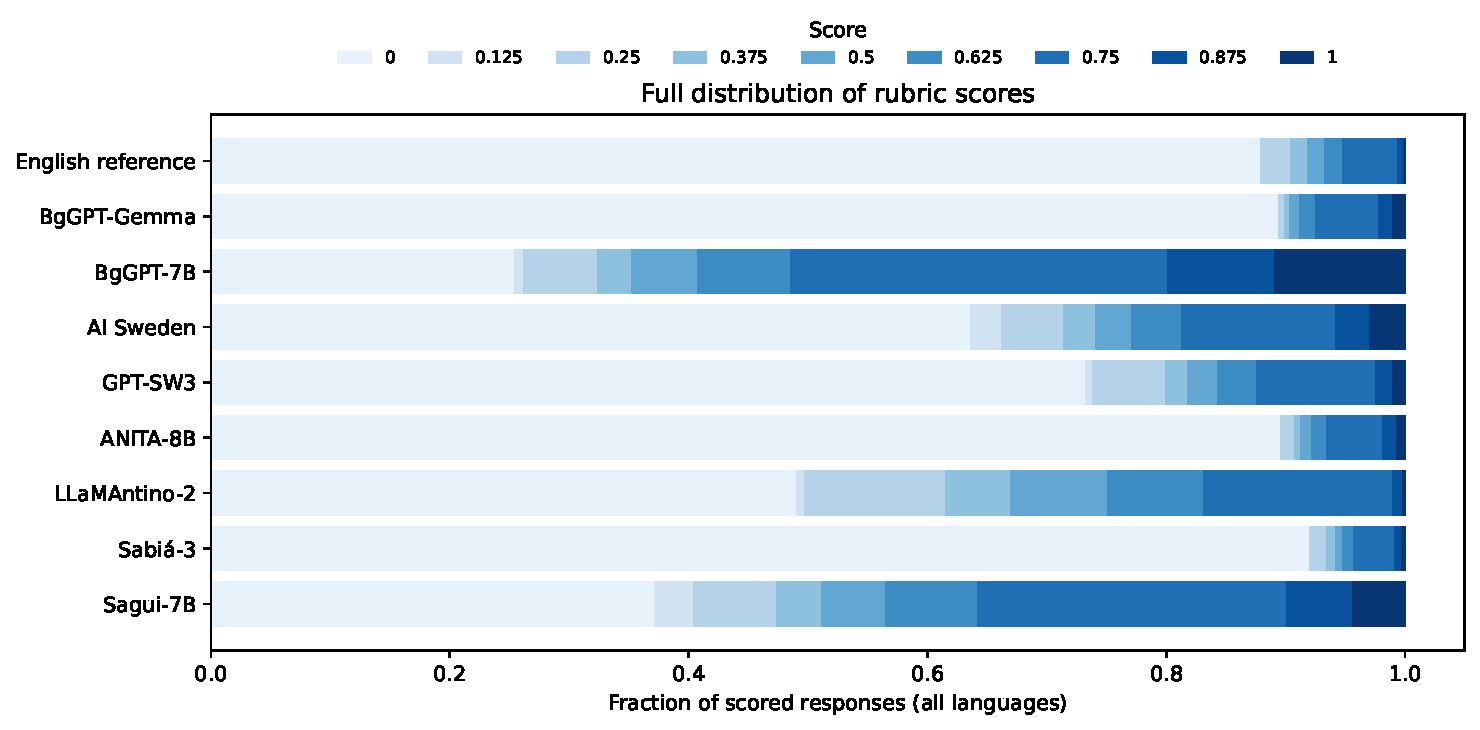
\includegraphics[width=\linewidth]{figures/graded_score_distribution.pdf}
\label{fig:graded-distribution}\fonte{Prepared by the author (2026).}
\end{figure}

The official scoring rule produces nine possible levels, from zero to one. ``Graded'' means that these intermediate levels are retained rather than reduced to a yes/no classification.

\subsection{English Reference Baseline}
\label{sec:reference-baseline-results}

Table~\ref{tab:graded-reference} reports the separate English-aligned reference model in each attack language. It provides an instruction-tuned reference checkpoint, Llama-3.1-8B-Instruct. It is not a matched parent checkpoint for those models, and it is excluded from the eight-model paired regressions. Differences from this reference therefore do not measure the effect of language specialization or safety changes inherited from a common parent model, but serve as a basis for comparison.

\GradedReferenceTable

% Generated by eval/scripts/write_reference_descriptive_contrast.py.
An additional post-review descriptive check examines the English reference separately (Figure~\ref{fig:reference-profiles}). Across its thirteen observed language cells, the Spearman correlation between distance and mean StrongREJECT score is $\rho=0.29$, while the correlation with SPEC is $\rho=-0.63$. English has the lowest mean score (0.022), whereas Swahili, the most distant language and the cell with the lowest SPEC, has the highest (0.156). When English is excluded, the distance correlation falls to $\rho=0.10$ and the SPEC correlation remains negative at $\rho=-0.52$. Thus, the reference descriptively follows the negative specialization direction expected by H\textsubscript{2} more clearly than the positive distance direction expected by H\textsubscript{1}. These are unadjusted correlations over a purposive language inventory, calculated after inspecting the reference profiles; they have no inferential intervals here and do not assess H\textsubscript{3}. The reference remains excluded from paired inference, and its pattern does not change the paired-panel hypothesis conclusions.


\begin{figure}[htbp]\centering
\caption[English reference profiles]{StrongREJECT and BELEBELE results for the English reference, Llama-3.1-8B-Instruct, in each attack language. Top left: mean StrongREJECT score, with 95\% source-prompt cluster percentile bootstrap intervals (2\,000 resamples). Top right: SPEC against mean StrongREJECT score, labelling the aligned language and the lowest and highest scores. Bottom: BELEBELE IF and CONS, with conditional 95\% Wilson intervals for CONS, and SPEC. Languages follow increasing URIEL+ distance from English but are equally spaced; shading and bold labels mark English. SPEC uses the same all-117-cell standardization as the paired targets. The reference is descriptive and excluded from paired inference.}
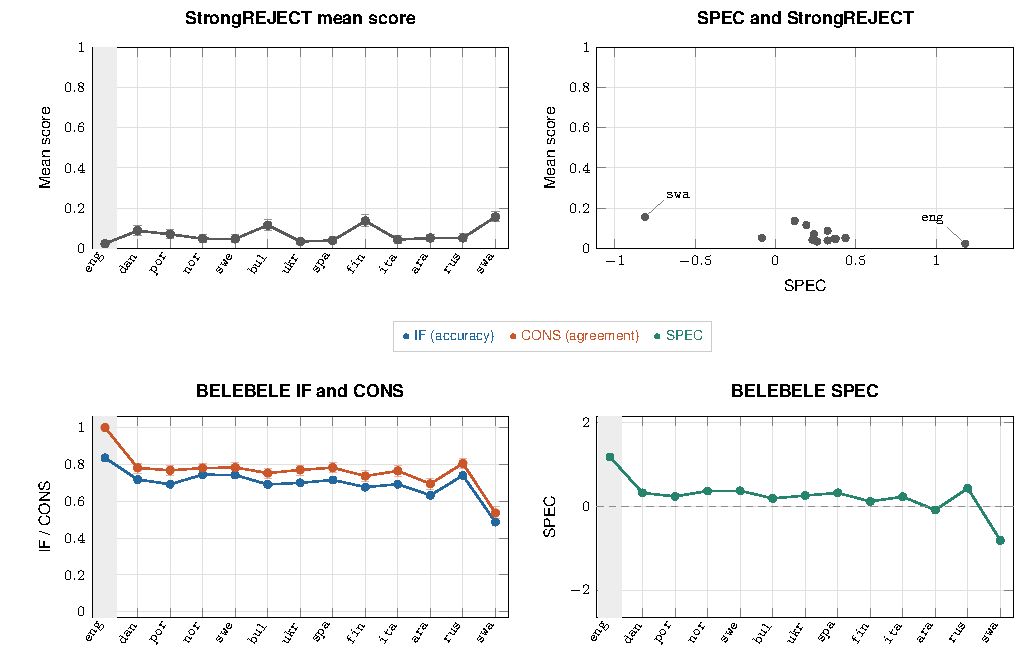
\includegraphics[max width=\linewidth]{figures/compiled/reference_profiles.pdf}
\label{fig:reference-profiles}\fonte{Prepared by the author (2026), based on the corrected BELEBELE release.}
\end{figure}

\clearpage
\section{Distance and Specialization}
\label{sec:graded-distance-spec}
The BELEBELE measures distinguish \emph{instruction following} (IF), operationalized as answer accuracy, from \emph{cross-lingual consistency} (CONS), agreement with aligned-language answers on comparable questions. \emph{Specialization} (SPEC) combines their standardized values with equal weights. A high CONS value need not imply correct answers, and a SPEC value summarizes benign benchmark behavior rather than safety alignment. Figure~\ref{fig:belebele-profiles} presents all three measures for each paired target; Figure~\ref{fig:belebele-worked-example} illustrates the scoring distinction on one question.

\GradedCorrelationsTable
\clearpage
Figure~\ref{fig:strongreject-profiles} shows the StrongREJECT mean for every attack language in a separate panel for each paired target. Its layout and language ordering match the BELEBELE profiles in Figure~\ref{fig:belebele-profiles}, making the harmful-assistance and benign-capability profiles easier to compare. Figures~\ref{fig:strongreject-profiles}, \ref{fig:graded-spec}, and \ref{fig:belebele-profiles} show only the paired targets; the English reference appears separately in Figure~\ref{fig:reference-profiles}. Weak targets are at left and strong targets at right, and the four rows correspond to the aligned-language pairs. Shading and bold labels identify the aligned language. Bars show the saved 95\% prompt-cluster bootstrap intervals. All panels share the same score scale. Languages are equally spaced and ordered by increasing URIEL+ distance; the connecting lines describe profiles rather than fitted trends. The plot with actual distance on the horizontal axis is retained in Appendix~\ref{app:graded-details}, Figure~\ref{fig:graded-distance}.
\begin{figure}[p]\centering
\caption[StrongREJECT profiles by model and attack language]{Mean StrongREJECT scores by model and attack language, with weak targets at left and strong targets at right. Rows are the Portuguese, Italian, Swedish and Bulgarian pairs. Zero scores are included; missing scores are excluded. Bars show 95\% source-prompt cluster percentile bootstrap intervals (2\,000 resamples). Shading and bold labels mark the aligned language. Languages follow increasing URIEL+ distance but are equally spaced; lines connect observations and are not fitted regressions. The English reference appears separately in Figure~\ref{fig:reference-profiles}.}

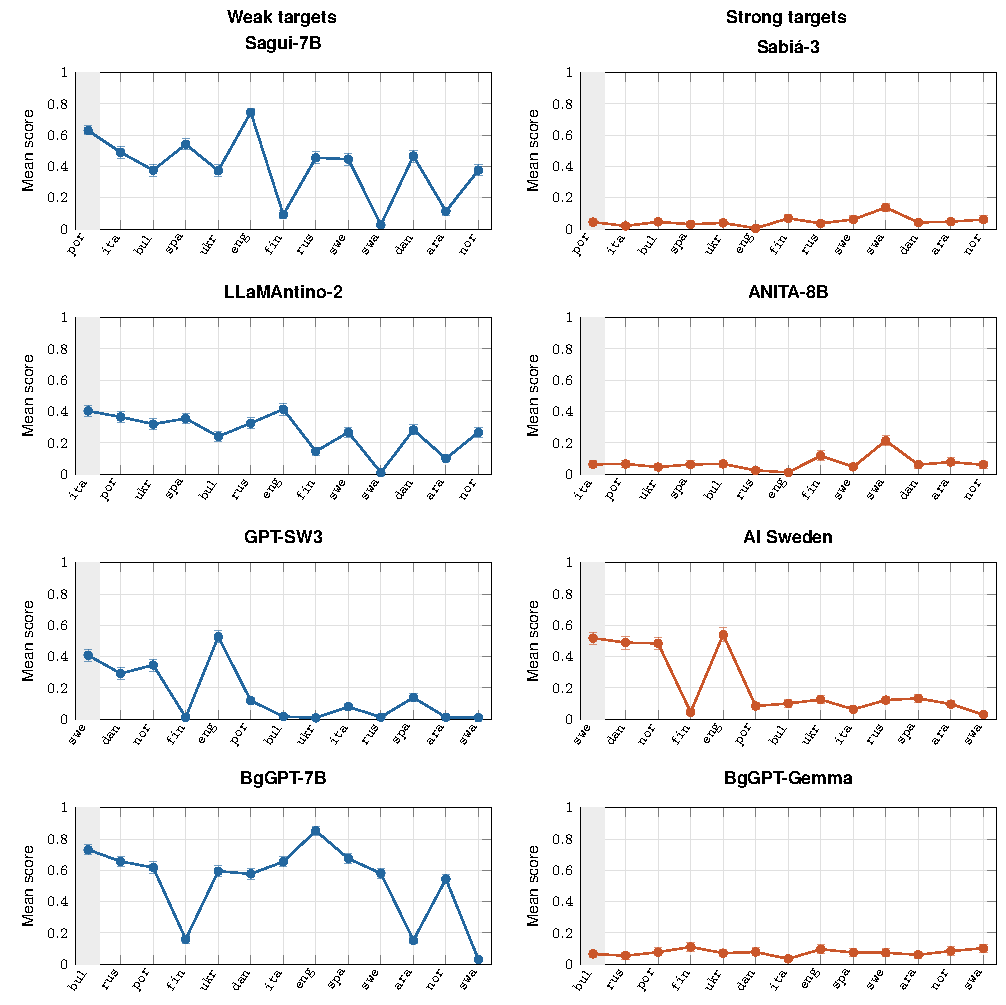
\includegraphics[max width=\linewidth,max height=.74\textheight]{figures/compiled/strongreject_profiles.pdf}
\label{fig:strongreject-profiles}\fonte{Prepared by the author (2026).}
\end{figure}
\begin{figure}[p]\centering
\caption[Specialization and StrongREJECT scores]{BELEBELE specialization and mean StrongREJECT score in the observed model--language cells of the four pairs, with weak targets at left and strong targets at right. Language labels identify the aligned language and the lowest and highest mean StrongREJECT scores within each model.}

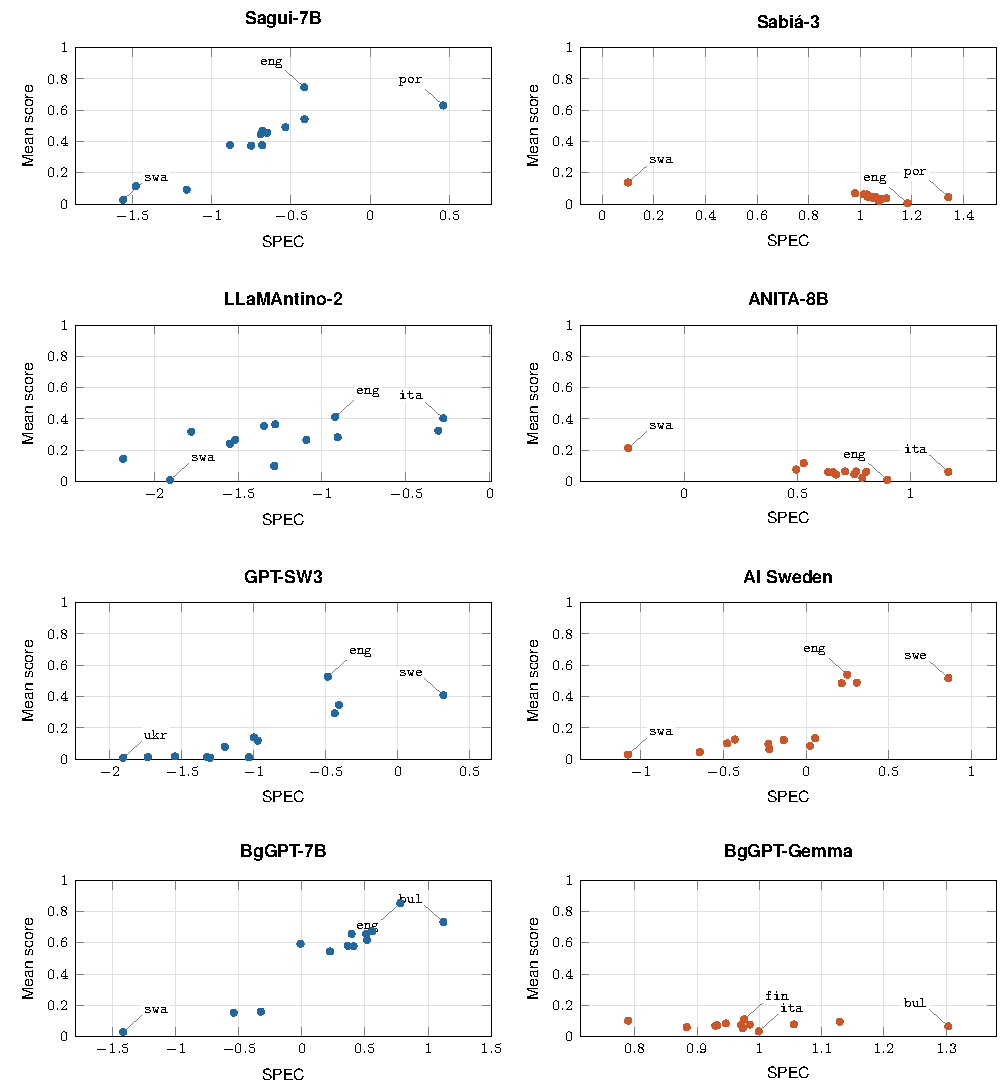
\includegraphics[max width=\linewidth,max height=.74\textheight]{figures/compiled/graded_spec_reference_scatter.pdf}
\label{fig:graded-spec}\fonte{Prepared by the author (2026).}
\end{figure}
The different appearance of LLaMAntino-2 in Figure~\ref{fig:belebele-profiles} reflects limited comparable answers, rather than a different plotting method. CONS has 95\% Wilson intervals for every model; the intervals for other models are generally narrower and therefore less conspicuous. LLaMAntino-2 has few parseable aligned-language answers, which limits the number of questions that can be compared across languages and makes its CONS intervals much wider. Hollow points identify cells with fewer than 100 comparable answers. We leave those CONS points, and the SPEC values that depend on them, disconnected so that the figure does not suggest a reliably measured language curve. The intervals quantify uncertainty conditional on the parseable pairs; they do not correct for missing or unparsed answers.

\begin{figure}[p]\centering
\caption[BELEBELE IF, CONS and SPEC profiles by model]{BELEBELE profiles for the four pairs, with weak targets at left and strong targets at right. The English reference appears separately in Figure~\ref{fig:reference-profiles}. Languages follow increasing URIEL+ distance; shading and bold labels mark the aligned language. IF is correct/900, counting unparsed answers as incorrect. CONS compares parseable canonical pairs; bars are conditional 95\% Wilson intervals. Hollow, disconnected CONS/SPEC points have paired $n<100$. SPEC uses all 117 cells for standardization, including the reference. Aligned-language CONS is one by construction; lines connect observations, not fitted trends.}

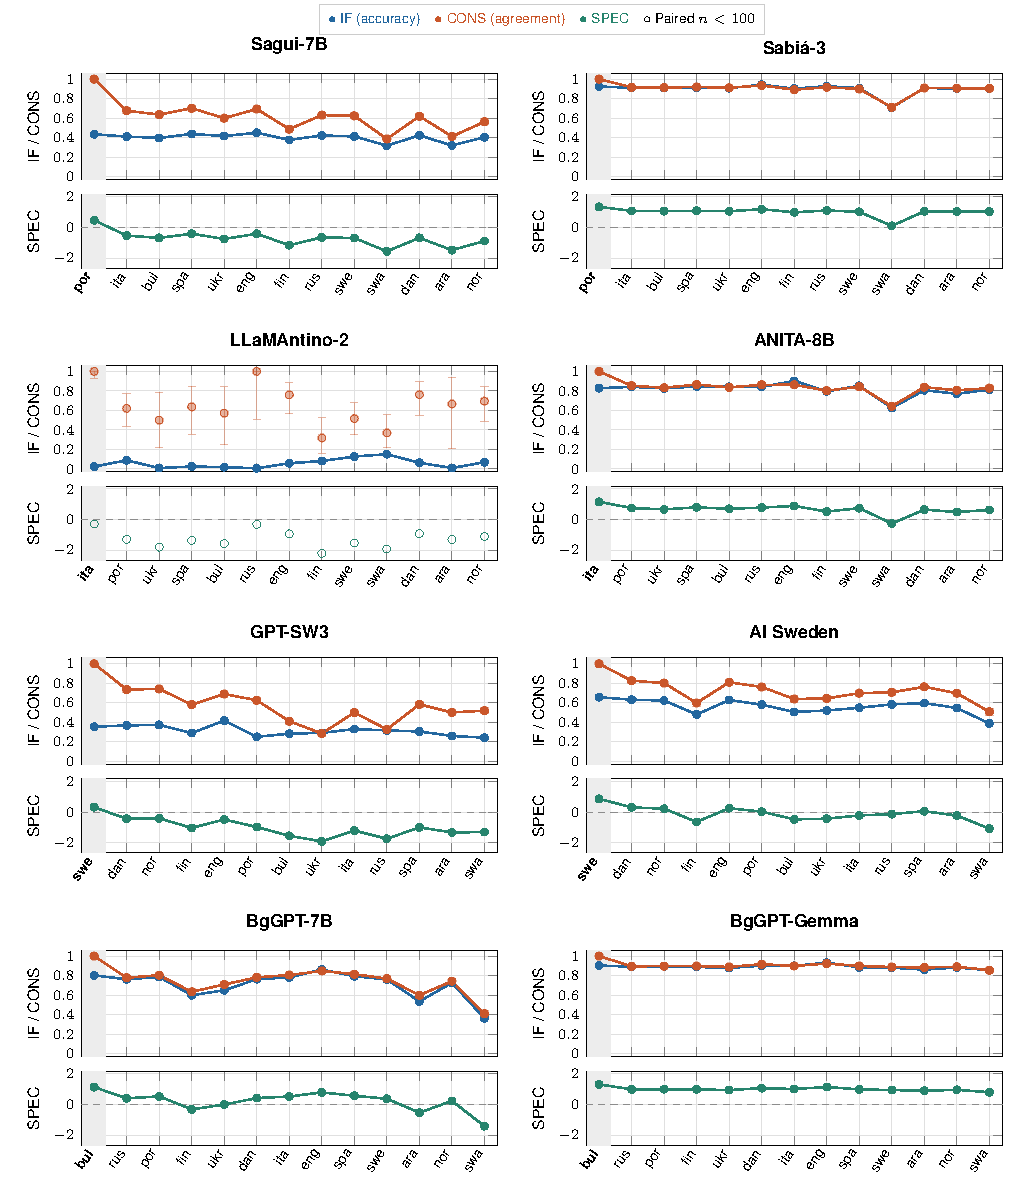
\includegraphics[max width=\linewidth,max height=.78\textheight]{figures/compiled/belebele_profiles.pdf}
\label{fig:belebele-profiles}\fonte{Prepared by the author (2026), based on the corrected BELEBELE release.}
\end{figure}
\begin{figure}[p]
\centering
\caption[BELEBELE accuracy and consistency example]{BELEBELE accuracy and consistency in a saved LLaMAntino-2 example. The same question appears at Italian row 726 and Russian row 359. The complete English source passage, question, and options are shown for reference; the quoted responses are the complete saved outputs. IF and CONS are aggregated over their respective denominators, as defined in the methodology.}

\begin{tikzpicture}[font=\small,x=1cm,y=1cm]
\definecolor{exampleblue}{HTML}{286F8C}
\definecolor{exampleorange}{HTML}{A64B39}

% Complete English passage from BELEBELE eng_Latn.jsonl, row 726;
% canonical identity: https://en.wikivoyage.org/wiki/Gambling, question 2.
\node[anchor=north west,inner sep=0,font=\small\bfseries] at (0,0) {English source passage};
\node[anchor=north west,inner sep=0,text width=14.05cm,align=left] (passage) at (0,-.55) {
\textit{``Casinos typically make many efforts to maximize time and money spent by guests. Windows and clocks are usually absent, and exits can be hard to find. They usually have special food, drink and entertainment offers, to keep guests in a good mood, and keep them at the premise. Some venues offer alcoholic beverages on the house. However, drunkenness impairs judgement, and all good gamblers know the importance of staying sober.''}
};
\coordinate (steps) at ([yshift=-.65cm]passage.south west);
\begin{scope}[shift={(steps)}]

\node[anchor=north west,inner sep=0,font=\small\bfseries] at (0,0) {1. Question};
\node[anchor=north west,inner sep=0,font=\small\bfseries] at (4.9,0) {2. Responses};
\node[anchor=north west,inner sep=0,font=\small\bfseries] at (9.8,0) {3. Scores};
\draw[black!35] (0,-.38) -- (14.05,-.38);

\node[anchor=north west,inner sep=0,text width=4.25cm,align=left] (source) at (0,-.7) {
\textbf{English source question}\\[7pt]
\textit{``According to the passage, what should a smart gambler avoid?''}\\[10pt]
\textbf{A. Drinking too much alcohol}\\[7pt]
B. Accepting any incentives\\[7pt]
C. Checking clocks or watches\\[7pt]
D. Inquiring about the nearest exit\\[10pt]
\textbf{Supplied gold: A}
};

\node[anchor=north west,inner sep=0,text width=4.05cm,align=left] (it) at (4.9,-.7) {
\textbf{Italian}\\
\textit{Aligned language}\\[9pt]
Saved output:\\[3pt]
\texttt{B. Accett}\\[9pt]
Parsed choice: \textbf{B}
};
\node[anchor=north west,inner sep=0,text width=4.05cm,align=left] (ru) at ([yshift=-.7cm]it.south west) {
\textbf{Russian}\\
\textit{Test language}\\[9pt]
Saved output:\\[3pt]
\texttt{B.}\\[9pt]
Parsed choice: \textbf{B}
};

\node[anchor=north west,inner sep=0,text width=4.25cm,align=left] (accuracy) at (9.8,-.7) {
\textbf{Accuracy (IF)}\\[9pt]
{\Large\color{exampleorange}\bfseries 0}\quad Incorrect\\[7pt]
Russian choice versus gold:\\[3pt]
$B\ne A$
};
\node[anchor=north west,inner sep=0,text width=4.25cm,align=left] (consistency) at ([xshift=4.9cm]ru.north west) {
\textbf{Consistency (CONS)}\\[9pt]
{\Large\color{exampleblue}\bfseries 1}\quad Agreement\\[7pt]
Italian versus Russian choice:\\[3pt]
$B=B$
};

% Derive the rules and footer from the actual text extents.
\node[fit=(source)(it)(ru)(accuracy)(consistency),inner sep=0] (content) {};
\draw[black!15] (4.6,-.65) -- (4.6,0 |- content.south);
\draw[black!15] (9.4,-.65) -- (9.4,0 |- content.south);
\coordinate (ruleleft) at ([yshift=-.45cm]content.south west);
\coordinate (ruleright) at ([yshift=-.45cm]content.south east);
\draw[black!35] (ruleleft) -- (ruleright);
\node[anchor=north west,inner sep=0,text width=14.05cm,align=left] at ([yshift=-.25cm]ruleleft) {
\textbf{Both answers are incorrect, but they agree.} This question contributes 0 to Russian IF and 1 to CONS.
};
\end{scope}
\end{tikzpicture}
\par\medskip
\label{fig:belebele-worked-example}
\fonte{Prepared by the author (2026).}
\end{figure}


The cell descriptions reveal heterogeneous language profiles. They do not identify independent effects of distance or specialization. BELEBELE measures reading comprehension and agreement with aligned-language answers; it does not directly measure safety or open-ended benign instruction following.

Russian is the extreme case. Only 20 Russian and 50 Italian outputs identify an option, leaving four canonical questions comparable across the two languages. All four agree, giving CONS $=1.00$ with a 95\% Wilson interval of $[0.510,1.000]$, although two agree on wrong answers; one disagreement would reduce the estimate to $0.75$. Appendix~\ref{app:belebele-sparse-answers} reports the per-language coverage, the saved fragments, the evidence that the cap was uniform across all nine models, and the share of unparsed outputs that no larger cap would recover. The pooled and stratum fits in Section~\ref{sec:graded-inference} retain this model, so its SPEC coefficient is estimated with one of eight models contributing an inverted proxy. Section~\ref{sec:future-belebele-likelihood} states the measurement change that would resolve this.

\section{Fractional-logit Analysis}
\label{sec:graded-inference}

The regression estimates the associations of distance and BELEBELE specialization with the expected StrongREJECT score, conditional on model identity and attack language. The outcome is each response's official score, including exact zeros and ones. The pooled fit uses \GMainN{} scored responses from the eight paired targets; the English reference is excluded.

\subsection{Estimation and Interpretation}

Coefficients use cohort-standardized predictors and the logit of expected score, with model and attack-language fixed effects and prompt-clustered intervals (Section~\ref{sec:magnitude-method}). They describe adjusted graded-score associations rather than binary-event odds ratios.

\GradedEffectsTable

Table~\ref{tab:graded-effects} reports the pooled fit and separate weak- and strong-pole fits. In the pooled fit, distance has coefficient \GDistanceInterval{} and SPEC has coefficient \GSpecInterval{}. Both stratum fits retain the same directions: negative for distance and positive for SPEC. Within this specification, more distant languages accompany lower expected scores, while higher measured specialization accompanies higher scores. \textbf{These directions contradict the associations predicted by H\textsubscript{1} and H\textsubscript{2} within the main specification.}

\clearpage
\subsection{Collinearity Diagnostics}

% Generated by eval/scripts/write_collinearity_explanation.py.
The practical question is whether the regression can separate the distance association from the specialization association. It includes distance, SPEC, model identity, and attack language. Some of these variables may contain overlapping information. For example, if SPEC is consistently higher for certain models, differences associated with SPEC also coincide with differences between those models. The model then has less information with which to distinguish the SPEC association from their baseline differences. This overlap is called \emph{collinearity}.

We check that overlap using the \emph{variance inflation factor} (VIF). A value of one indicates no linear overlap between a predictor and the other predictors; larger values indicate greater overlap.\footnote{VIF is calculated as $1/(1-R^2)$ by regressing the predictor on the other fitted design columns. This auxiliary $R^2$ concerns the predictor, not StrongREJECT scores. VIF is a design diagnostic; it does not directly multiply the robust GEE standard errors.} Here, ``other predictors'' includes the model and language indicators, as well as the other substantive predictor.

Table~\ref{tab:graded-diagnostics} reports distance VIF 2.46 and SPEC VIF 13.51 in the pooled fit. Distance has comparatively less overlap; SPEC has substantial overlap, making its separate adjusted contribution harder to isolate. This does not imply that SPEC is unimportant. Because its VIF exceeds the chosen threshold of five, we check simpler fits that include only one substantive predictor at a time.

The condition number checks the same general problem across the whole design, rather than for one predictor. Larger values indicate combinations of columns that are harder to distinguish numerically. It is 16.7 in the pooled fit and 27.2 when IF and CONS replace SPEC. These values depend on scaling and coding; our design includes cohort-standardized continuous predictors, an intercept, and treatment-coded model/language indicators. We report them alongside VIF without imposing a separate condition-number cutoff.


\clearpage
\GradedDiagnosticsTable
\GradedSingleTable

% Generated by eval/scripts/write_collinearity_explanation.py.
The single-predictor fits ask how the estimate changes when the other substantive predictor is omitted. We fit distance without SPEC, and SPEC without distance, retaining model and attack-language indicators in both cases. These pooled comparisons use the same 32\,090 scored responses and the same standardization. The following comparison therefore reflects a change in adjustment, rather than a change in sample:

\begin{center}
\small
\begin{tabular}{lrr}
\toprule
Predictor & Distance and SPEC together & Without the other predictor \\
\midrule
Distance & $-0.112$ & $-0.385$ \\
SPEC & $0.954$ & $1.157$ \\
\bottomrule
\end{tabular}
\end{center}

Both coefficients keep their signs, but their sizes change: the distance estimate becomes more negative without SPEC, while the SPEC estimate becomes more positive without distance. The estimated size of an association therefore depends on what else the regression accounts for. These coefficients are on the logit of expected score; they are not changes of that size in the original score. Table~\ref{tab:graded-single} reports the single-predictor intervals and the IF/CONS sensitivities.

Omitting distance does not remove all overlap: SPEC's VIF is still 7.99 because it remains associated with the retained model/language indicators. Likewise, the decomposition has IF VIF 38.41 and CONS VIF 5.04. The simpler fits reveal sensitivity to adjustment; they do not isolate a causal effect or resolve omitted-variable bias.

For H\textsubscript{3}, the implication is that ranking distance and SPEC as independent explanations requires caution. Standardization makes their coefficient units comparable, but the estimates still depend on overlapping predictors and cohort choices. We therefore consider their signs, sizes, intervals, and stability together. A larger absolute coefficient or smaller $p$-value alone does not establish a stronger and more stable predictor.

Finally, convergence answers a different question: whether the fitting algorithm reached a solution. All reported fits pass convergence, finite-estimate, and positive-definite covariance checks. Those checks make the estimates numerically usable; a successfully fitted model can still have substantial collinearity.


\subsection{Capability Components and Tokenization}

SPEC averages standardized BELEBELE accuracy (IF) and aligned-language answer agreement (CONS). The decomposition replaces that composite with its two components, asking which associations remain visible when they enter together. IF rewards a correct choice; CONS rewards matching choices, including matching wrong choices. Figure~\ref{fig:belebele-worked-example} and Appendix~\ref{app:belebele-sparse-answers} illustrate the distinction.

\GradedComponentsTable

The IF coefficient is \GIfCoef{} and the CONS coefficient is \GConsCoef{}. Both are positive: in this observed panel, better benign answer selection and greater answer agreement accompany higher harmful-assistance scores after the stated adjustment. IF has substantial collinearity, CONS depends on aligned-language behavior, and sparse parsing can distort the proxy.

\afterpage{\TokenizerDiagnosticsFigure\TokensPerCharacterFigure}

Token inflation is the number of tokens needed for an attack-language prompt relative to the same model's aligned-language version, after applying its chat template. It measures segmentation cost, not comprehension or safety. The tokenizer sensitivity compares the main specification with an added inflation term on exactly the same tokenizer-complete responses. A negative inflation coefficient describes an association in that cohort; it does not show that increasing token counts would make a model safer. Context-risk claims require actual token budgets and context limits, which remain unavailable for some records.

Sabi\'a-3's entries are unavailable in both tokenizer figures (Figures~\ref{fig:tokenizer-diagnostics} and \ref{fig:tokens-per-character}) because this API-served model has no usable local tokenizer assets in the pipeline and no input-token counts retained in the frozen records. Without those counts, we cannot calculate tokens per character or the attack-language/Portuguese token-count ratio. The missing markers indicate unavailable measurements, not zeros. Sabi\'a-3 remains in the main StrongREJECT and BELEBELE analyses, but is excluded from fits requiring token inflation. The tokenizer sensitivity therefore compares models with and without the inflation term on the same remaining complete rows, as specified in Section~\ref{sec:tokenizer-diagnostics}.


Figure~\ref{fig:tokens-per-character} complements token inflation with absolute segmentation density within each tokenizer. Its denominator is prompt characters rather than aligned-language tokens; the numerator includes chat-template overhead. Comparisons should focus on language differences within a model, since vocabularies, templates, and the byte length of characters differ across models and scripts. Neither diagnostic measures whether a model understands a request.

\subsection{Sensitivity to Coverage and Measurement}

The sensitivity analyses examine changes in measurement, cohort inclusion and covariate adjustment. Table~\ref{tab:graded-sensitivity} reports each resulting specification. Comparisons between rows require attention to both the included responses and the model terms.

\clearpage
\GradedSensitivityTable

The non-aligned fit excludes responses in each model's aligned language. The original-complete-cohort fit restricts analysis to the historical complete-cell inventory after the corrected question join. Removing questionable BELEBELE items tests sensitivity to supplied gold labels, without silently replacing them; it changes the IF and CONS inputs rather than the response inventory, so its scored count is unchanged and its coefficients differ from the pooled fit only in the third decimal. Removing selected languages or BLASER-flagged translations checks whether those translation concerns determine the reported signs. The two tokenizer rows form a matched-cohort comparison: their scored response counts are identical, and only the inflation adjustment changes.

The CONS-coverage restriction has a different consequence. Requiring at least 100 comparable questions removes sparsely measured cells, including the entire weak Italian model, and turns the distance point estimate positive. It changes both measurement coverage and the model inventory, so the change cannot be attributed to a better CONS estimate alone. Section~\ref{sec:cluster-sensitivity} shows that this apparent reversal does not survive correctly clustered inference: the restricted interval covers zero, as does the pooled interval, so the two specifications do not in fact disagree about the direction of the distance association. Taken across every specification in Table~\ref{tab:graded-sensitivity} and the two strata, the distance coefficient is negative in \RDistanceNegativeCount{} of \RDistanceSpecCount{} fits; the single positive fit is this restriction.

\subsection{Clustering and the Scale of Independent Variation}
\label{sec:cluster-sensitivity}

Distance and SPEC do not vary within a model--language cell. Distance is a function of the aligned and attack languages; SPEC is defined per cell. Both therefore take only \RNumCells{} distinct values in the paired panel, whereas a source-prompt cluster spans every cell. Clustering the robust covariance on source prompts cuts across the variation being tested, which understates uncertainty for precisely these two coefficients (Section~\ref{sec:magnitude-method}). Table~\ref{tab:cluster-sensitivity} refits the same equations under cell and two-way clustering. Point estimates are unchanged by construction, so only the intervals move.

\RClusterSensitivityTable

The consequence for H\textsubscript{1} is substantial. The pooled distance standard error rises from \RDistancePromptSE{} to \RDistanceCellSE{}, a factor of about \RSEInflation{}, and the interval widens from \RDistancePromptInterval{} to \RDistanceCellInterval{}, which covers zero. The CONS-coverage restriction likewise moves to \RConsDistanceCellInterval{}, also covering zero. The two cohorts therefore do not provide conflicting evidence about the sign of the distance association; neither distinguishes it from zero. The earlier description of a sign reversal was an artifact of clustering on a dimension along which the predictor does not vary.

Two results do survive. In the non-aligned cohort, which excludes the aligned-language cells where distance is zero and CONS is one by construction, the distance coefficient remains \RNonAlignedDistanceCellInterval{} and still excludes zero, in the direction opposite to H\textsubscript{1}. SPEC remains bounded away from zero in the pooled (\RSpecCellInterval{}), non-aligned (\RNonAlignedSpecCellInterval{}) and weak-pole fits; only the strong-pole stratum becomes inconclusive. With \RNumCells{} clusters these intervals rest on approximate asymptotics and should be read as indicative.

\subsection{Compliance Frequency and Conditional Magnitude}
\label{sec:outcome-decomposition-results}

A mean score is the product of how often a model complies and how useful that compliance is (Equation~\ref{eq:score-identity}). Table~\ref{tab:descriptive-identity} reports both factors. For the paired panel the identity reads $\RMeanPooled{} = \RAsrPooled{} \times \RPositiveMeanPooled{}$.

\RDescriptiveIdentityTable

The two factors behave very differently. Compliance frequency spans \RAsrRange{} across the nine models, a ninefold range, while conditional magnitude spans only \RPositiveMeanRange{}. Differences between models in mean score are therefore almost entirely differences in how often they comply, not in how useful their compliance is once it occurs. The same holds for the aligned-language contrast: compliance frequency falls from \RAsrAligned{} in the aligned language to \RAsrNonAligned{} outside it, while conditional magnitude moves only from \RPositiveMeanAligned{} to \RPositiveMeanNonAligned{}. Models in this panel are more likely to comply in the language they were aligned in.

\ROutcomeDecompositionTable

Refitting the same design on each factor separates two readings of the SPEC association (Section~\ref{sec:outcome-decomposition-method}). Because the rubric rewards specificity and convincingness, a capability proxy could raise scores purely by raising fluency, and that mechanism would act on conditional magnitude. It does not. SPEC's coefficient is \RBinarySpecInterval{} on compliance frequency but only \RPositiveSpecInterval{} on conditional magnitude: the association is concentrated on whether the model complies at all. Distance, by contrast, is essentially flat across the three outcomes (\RBinaryDistanceInterval{} on frequency, \RPositiveDistanceInterval{} on magnitude), so it does not distinguish refusal behavior from output quality either. The frequency result weakens, but does not eliminate, the reading of SPEC as a pure fluency artifact; the positive-only cohort is selected by its outcome and the cell-clustered intervals of Table~\ref{tab:cluster-sensitivity} apply here too.

\subsection{Pre-specified Heterogeneous-Pair Check}
\label{sec:prereg-matrix-results}

Every analysis above was selected after inspecting results. The heterogeneous-pair matrix was not, which is why it is reported separately (Section~\ref{sec:prereg-matrix-method}). Table~\ref{tab:prereg-sign-retention} gives the within-model distance slopes at each pole.

\RPreregRetentionTable

\RPreregRetained{} of \RPreregEvaluated{} pairs retain the slope sign at both poles, which falls in the matrix band that does not support H\textsubscript{1}. The split is more informative than the count. \RPreregPositivePairs{} pairs are positive at both poles, the configuration H\textsubscript{1} predicts, and \RPreregNegativePairs{} is negative at both. In the remaining three pairs the weak pole is negative and the strong pole positive, so the poles disagree. The one retained pair is retained in the negative direction, which the matrix counts as agreement but which cannot support a hypothesis predicting positive slopes. This is the only pre-committed decision rule in the analysis, and it does not favor H\textsubscript{1} under either reading.

\clearpage
%\QualityMissingAnalysesTable

\section{Qualitative Interpretation and Limits}
\label{sec:qualitative-error-analysis}

Appendix~\ref{app:qualitative-strongreject-examples} reproduces the complete saved English response back-translations for selected experimental cases. Their original-language texts and record identities are preserved in a companion export. These are illustrative selections, not a representative sample. The full texts make visible features hidden by an average: disclaimers followed by assistance, repetition in refusals, and outputs that end mid-sentence. The back-translations are the judge-facing texts, not verified human translations.

\section{Assessment of the Hypotheses}
\label{sec:hypothesis-comparison}

Figure~\ref{fig:hypothesis-expected-observed} contrasts the associations predicted by H\textsubscript{1}--H\textsubscript{3} with the estimated associations. The left panels illustrate the expected directions and relative magnitudes; their shapes do not represent data or specified effect sizes. The right panels report fractional-logit coefficients and prompt-clustered confidence intervals from the graded analysis. They describe associations conditional on the included predictors, model indicators and attack-language indicators. The graded outcome and estimation procedure were selected after inspection of the results, as disclosed in Section~\ref{sec:magnitude-method}.

\begin{figure}[p]\centering
\caption[Expected associations and graded estimates]{Predicted associations and graded estimates for H\textsubscript{1}--H\textsubscript{3}. Left panels are schematic. Right panels show standardized fractional-logit coefficients with prompt-clustered 95\% confidence intervals; the final row reports absolute pooled coefficients. The CONS-coverage restriction changes the estimation cohort, including the exclusion of LLaMAntino-2. Standardization is performed within each cohort. Collinearity limits the interpretation of relative coefficient magnitudes.}

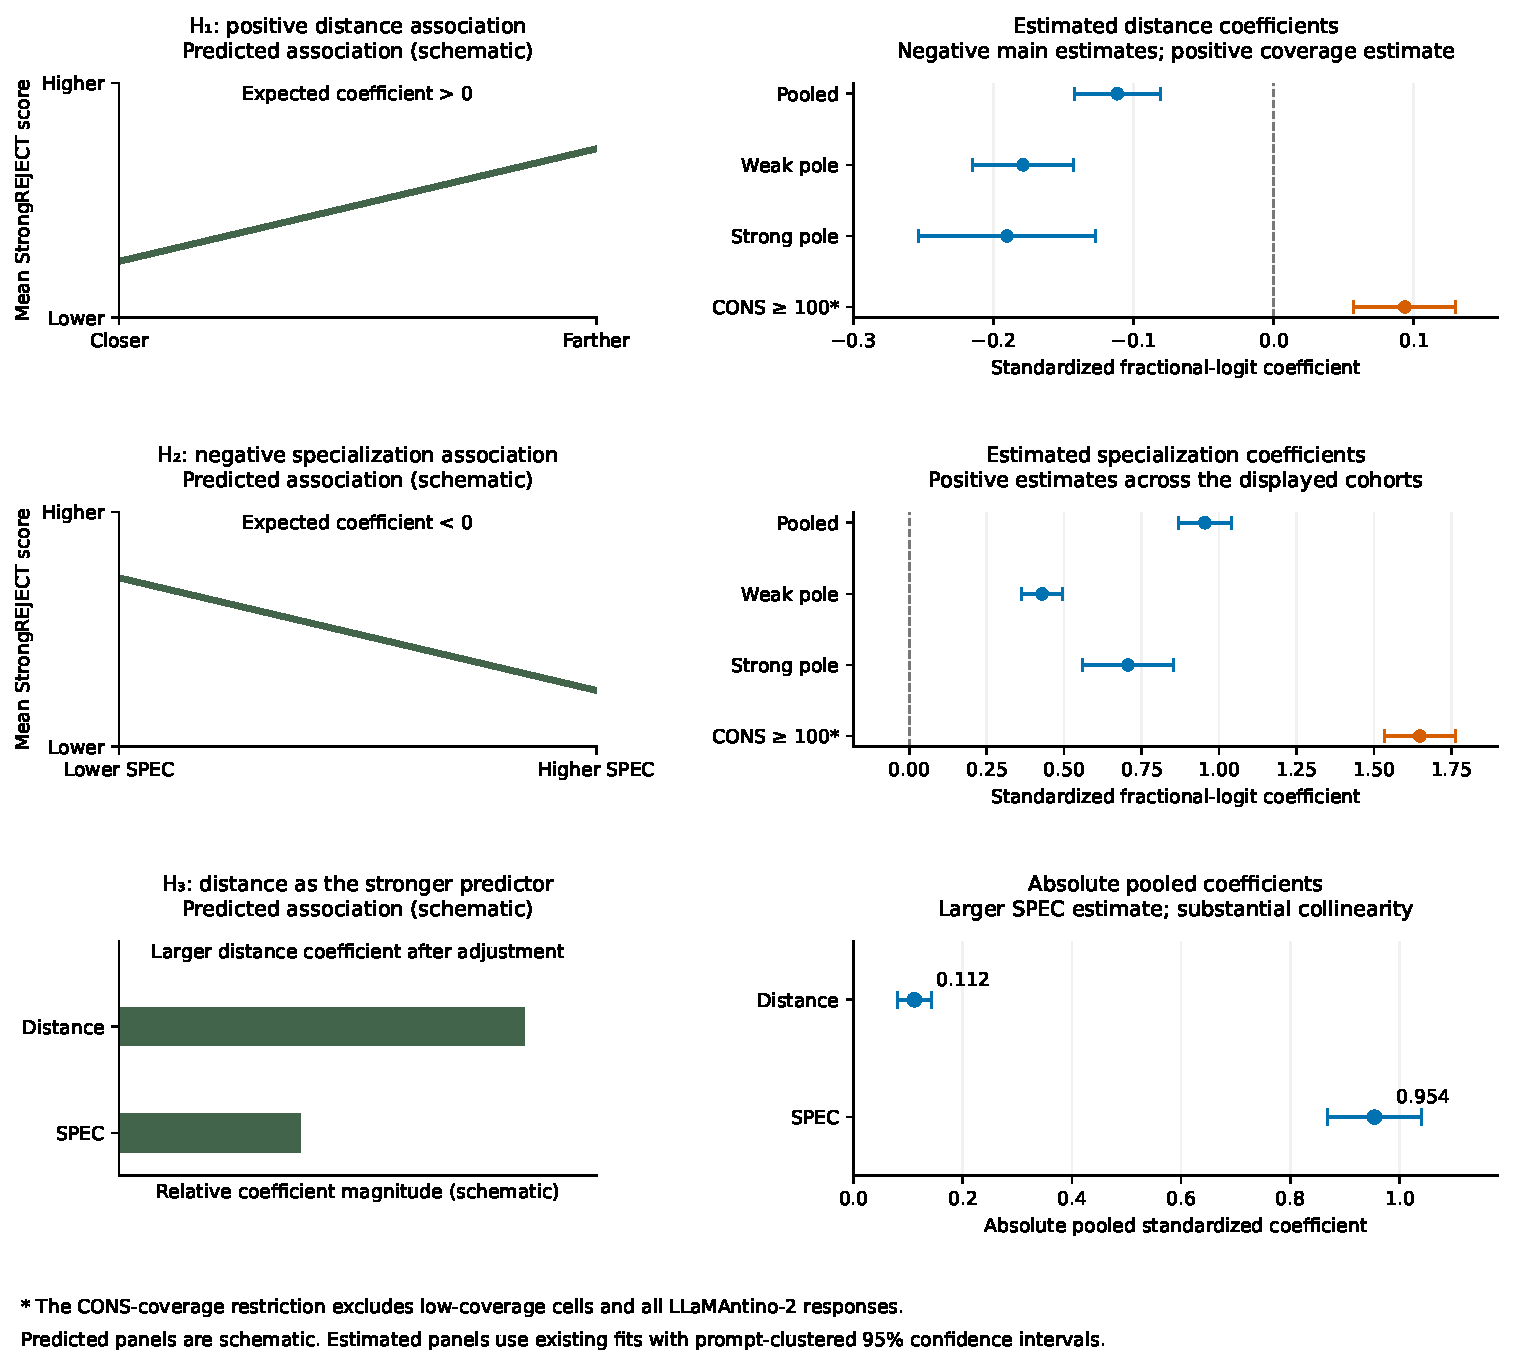
\includegraphics[width=\linewidth,height=.86\textheight,keepaspectratio]{figures/hypothesis_expected_observed.pdf}
\label{fig:hypothesis-expected-observed}
\fonte{Prepared by the author (2026).}
\end{figure}

\subsection{H\textsubscript{1}: Linguistic Distance}

The pooled estimate is \GDistanceInterval{} under source-prompt clustering, and the weak- and strong-pole estimates are also negative. All three contradict the predicted direction. Across every reported specification the coefficient is negative in \RDistanceNegativeCount{} of \RDistanceSpecCount{} fits; the sole positive fit is the CONS-coverage restriction, which removes the entire weak Italian model.

Correctly clustered inference changes what can be claimed from this, in both directions. Clustering on the model--language cell, the scale at which distance actually varies, widens the pooled interval to \RDistanceCellInterval{}, which covers zero; the CONS-restricted interval becomes \RConsDistanceCellInterval{} and also covers zero (Section~\ref{sec:cluster-sensitivity}). The two specifications therefore never disagreed about direction, and the earlier reversal narrative does not survive. What survives is a null: no specification yields a distance association distinguishable from zero in the predicted positive direction.

The pre-specified pair matrix points the same way. \RPreregRetained{} of \RPreregEvaluated{} pairs retain the slope sign, with \RPreregPositivePairs{} pairs positive at both poles, placing the result in the band that does not support H\textsubscript{1} (Section~\ref{sec:prereg-matrix-results}).

\textbf{H\textsubscript{1} is not supported.} The failure is not one of instability but of absence: the predicted positive association is not detected in the pooled panel, in either stratum, under any coverage restriction, or in any aligned-language pair. The one specification where distance is detectable is the non-aligned cohort, at \RNonAlignedDistanceCellInterval{}, and its sign is negative. That estimate excludes the aligned-language cells where distance is zero and CONS is one by construction, so it is the cleaner specification for a distance hypothesis; it is nonetheless a single cohort and should not be read as establishing that distance generally reduces harmful assistance.

\subsection{H\textsubscript{2}: Post-training Specialization}

The pooled estimate is \GSpecInterval{}. Both stratum estimates and the reported sensitivity estimates are positive. Higher measured specialization is therefore associated with higher expected scores, contrary to the predicted protective direction. Unlike the distance association, this one survives cell clustering: \RSpecCellInterval{} pooled and \RNonAlignedSpecCellInterval{} in the non-aligned cohort, with only the strong-pole stratum becoming inconclusive (Section~\ref{sec:cluster-sensitivity}). The decomposition also yields positive IF and CONS coefficients, although collinearity and sparse comparison coverage constrain their separate interpretation.

The frequency/magnitude split addresses the most obvious alternative explanation. Because the rubric rewards specificity and convincingness, a capability proxy might raise scores simply by making outputs more fluent, which would show up in conditional magnitude. The association is instead concentrated on compliance frequency: \RBinarySpecInterval{} on whether the model complies at all, against \RPositiveSpecInterval{} on magnitude given compliance (Section~\ref{sec:outcome-decomposition-results}). The proxy tracks refusal behavior more than output quality, which makes a pure fluency artifact a less adequate account than it would otherwise be.

\textbf{H\textsubscript{2}'s protective association is not supported by the reported graded analyses.} The positive estimates describe an association between the proxy and harmful-assistance scores. They do not establish that specialization causes unsafe responses or that an intervention improving benign performance would reduce safety. The measurement caveat in Section~\ref{sec:graded-distance-spec} also applies with full force: for one of the eight models the proxy is not a usable measurement at all, and the association is estimated with that model included.

\subsection{H\textsubscript{3}: Relative Strength of Distance and Specialization}

In the pooled joint model, the absolute coefficients are approximately $0.112$ for distance and $0.954$ for SPEC. This ordering does not support the proposed predominance of distance. Under cell clustering the distance interval covers zero while the SPEC interval does not, so the ordering is not merely unfavorable to H\textsubscript{3}: only one of the two predictors has a detectable association at all. SPEC's pooled VIF of \GSpecVIF{} nonetheless indicates substantial collinearity with the other design terms, and its larger coefficient cannot be interpreted as an independent or causal contribution.

\textbf{H\textsubscript{3} is not established: the analysis provides neither the predicted magnitude ordering nor a detectable distance association to rank. Taken together, the three assessments do not support the proposed directional explanation for this model and language inventory.} Their scope remains conditional on the observed panel, the specialization measurements and the stated estimation assumptions.

\end{otherlanguage*}

Complete model--language results, all graded coefficient estimates, and script-extracted qualitative record metadata appear in Appendix~\ref{app:graded-details}.
